\documentclass[11pt,a4paper]{article}
\usepackage[utf8]{inputenc}
\usepackage[T1]{fontenc}
\usepackage[spanish,es-noshorthands]{babel}
\usepackage{lmodern,microtype,graphicx,booktabs,tabularx,xcolor,amsmath,amssymb,float}
\usepackage[margin=2.2cm]{geometry}
\usepackage[most]{tcolorbox}
\usepackage[hidelinks]{hyperref}
\usepackage{fancyhdr}
\definecolor{navy}{HTML}{12263A}\definecolor{teal}{HTML}{0F766E}\definecolor{nar}{HTML}{E8772E}
\pagestyle{fancy}\fancyhf{}
\fancyhead[L]{\small\color{teal} Control y gemelo digital del brazo XK-JS1-1}
\fancyhead[R]{\small\color{teal} Presentación del 28/11/2026}
\fancyfoot[C]{\small\thepage}
\renewcommand{\headrulewidth}{0.4pt}
\setlength{\parindent}{0pt}\setlength{\parskip}{6pt}
\newtcolorbox{guion}[1]{enhanced,breakable,colback=teal!6,colframe=teal,boxrule=0.8pt,arc=2pt,
  title={\textbf{Guion} \hfill #1},fonttitle=\small\bfseries,coltitle=white,colbacktitle=teal}
\newtcolorbox{nota}{enhanced,breakable,colback=nar!8,colframe=nar,boxrule=0.8pt,arc=2pt}
\newcommand{\codigo}[1]{\texttt{#1}}
\begin{document}

\begin{titlepage}
\centering
{\large\color{navy} UNIVERSIDAD MAYOR DE SAN ANDRÉS\\ FACULTAD DE INGENIERÍA · INGENIERÍA ELECTRÓNICA\par}
\vspace{1.6cm}
{\color{nar}\bfseries MUESTRA DEL TRABAJO · MENCIÓN CONTROL\par}
\vspace{0.4cm}
{\Huge\bfseries\color{navy} Control y gemelo digital\\[4pt] del brazo robótico XK-JS1-1\\[4pt] de 4 grados de libertad\par}
\vspace{0.6cm}
{\Large Documento de la presentación: diapositivas, explicación y guion\par}
\vspace{1cm}
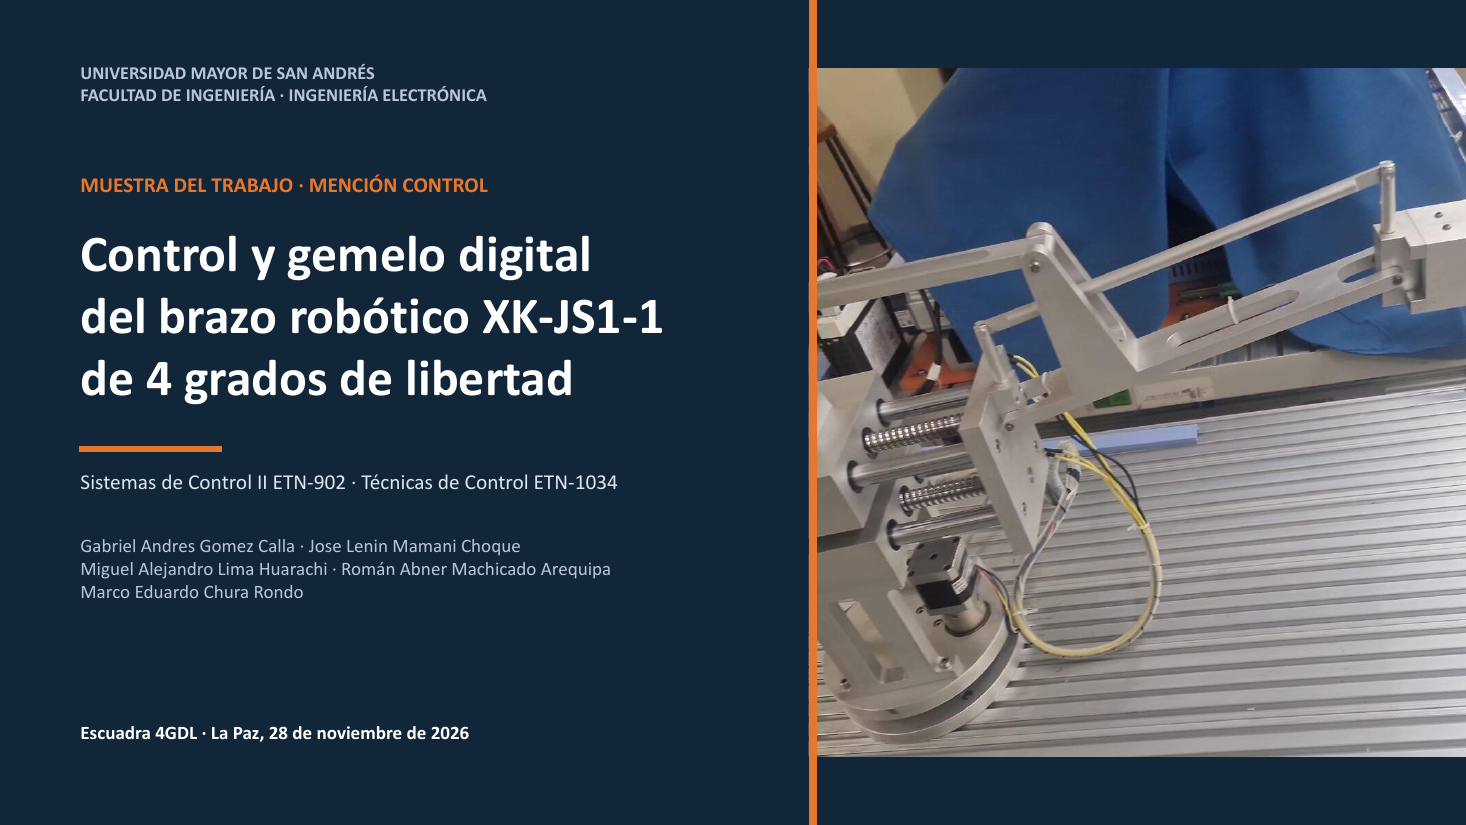
\includegraphics[width=0.75\linewidth]{laminas/l-01.png}\par
\vspace{1cm}
{\large Sistemas de Control II ETN-902 · Técnicas de Control ETN-1034\par}
\vspace{0.6cm}
Gabriel Andres Gomez Calla · Jose Lenin Mamani Choque\\
Miguel Alejandro Lima Huarachi · Román Abner Machicado Arequipa\\
Marco Eduardo Chura Rondo\par
\vfill
{\bfseries Escuadra 4GDL · La Paz, 28 de noviembre de 2026\par}
\end{titlepage}

\tableofcontents
\clearpage

\section{Cómo usar este documento}
Este documento acompaña a la presentación de unos 15 minutos sobre el trabajo realizado en el brazo XK-JS1-1,
con el enfoque de la mención de control. Para cada diapositiva se incluye la imagen, una explicación de lo que
muestra (para estudiar el contenido) y un \textbf{guion} con lo que se dice y el tiempo que le corresponde. El
mismo guion está en las notas del orador de la presentación de Google Slides y del archivo PowerPoint.

Después de las diapositivas hay dos capítulos de apoyo: el gemelo digital en detalle (para responder preguntas)
y la guía paso a paso de la demostración, con la habilitación de los observadores libres.

\begin{center}\small
\begin{tabularx}{\linewidth}{c X c r}
\toprule
\textbf{N.º} & \textbf{Lámina} & \textbf{Tiempo} & \textbf{Duración}\\
\midrule
01 & Control y gemelo digital del brazo XK-JS1-1 & 0:00--0:30 & 30 s\\
02 & De una maqueta sin documentación a una planta modelada y supervisada & 0:30--1:15 & 45 s\\
03 & Brazo XK-JS1-1: tres ejes con motores paso a paso y una garra & 1:15--2:15 & 60 s\\
04 & P\&ID ISA-5.1: cinco lazos, uno por función & 2:15--2:55 & 40 s\\
05 & Esquema eléctrico IEC 60617 y mapa de entradas/salidas & 2:55--3:35 & 40 s\\
06 & Control de posición en lazo abierto con trenes de pulsos & 3:35--4:35 & 60 s\\
07 & Modelo identificado: integrador con tiempo muerto por eje & 4:35--5:35 & 60 s\\
08 & Controlabilidad y observabilidad: el hardware limita el control & 5:35--6:20 & 45 s\\
09 & PI discreto por asignación de polos (listo para cuando haya sensor) & 6:20--7:20 & 60 s\\
10 & LQR: qué se puede con el hardware actual y con el propuesto & 7:20--8:05 & 45 s\\
11 & Cinemática: de los carros a la posición de la garra & 8:05--8:35 & 30 s\\
12 & Gemelo digital: una réplica virtual sincronizada con el PLC real & 8:35--9:35 & 60 s\\
13 & Cómo funciona: el ciclo de lectura, cálculo y mando & 9:35--10:35 & 60 s\\
14 & Acceso por red: operadores, observadores y observadores libres & 10:35--11:25 & 50 s\\
15 & Supervisión: telemetría, indicadores e integración industrial & 11:25--11:55 & 30 s\\
16 & Demostración: la app del gemelo en funcionamiento & 11:55--13:55 & 120 s\\
17 & Resultados, limitaciones y trabajo futuro & 13:55--14:40 & 45 s\\
18 & Gracias $\cdot$ Preguntas & 14:40--14:50 & 10 s\\
\midrule
 & \textbf{Total} & & \textbf{14:50}\\
\bottomrule
\end{tabularx}
\end{center}

\begin{nota}
\textbf{Reparto sugerido del tiempo.} Introducción (láminas 1--2): 1:15 · planta e instrumentación (láminas 3--5): 2:20 · estructura de control y
modelo (6--8, 11): 3:15 · diseño de controladores (9--10): 1:45 · gemelo digital (12--15): 3:20 ·
demostración (16): 2:00 · cierre (17--18): 0:55. Si el tiempo apremia, las láminas 5 y 11 se pueden pasar
en 15~s cada una; la demostración no se debe recortar.
\end{nota}
\clearpage

\section{Las diapositivas, explicadas}

\section*{Lámina 01 · Control y gemelo digital del brazo XK-JS1-1}
\addcontentsline{toc}{subsection}{Lámina 01 · Control y gemelo digital del brazo XK-JS1-1}
\begin{center}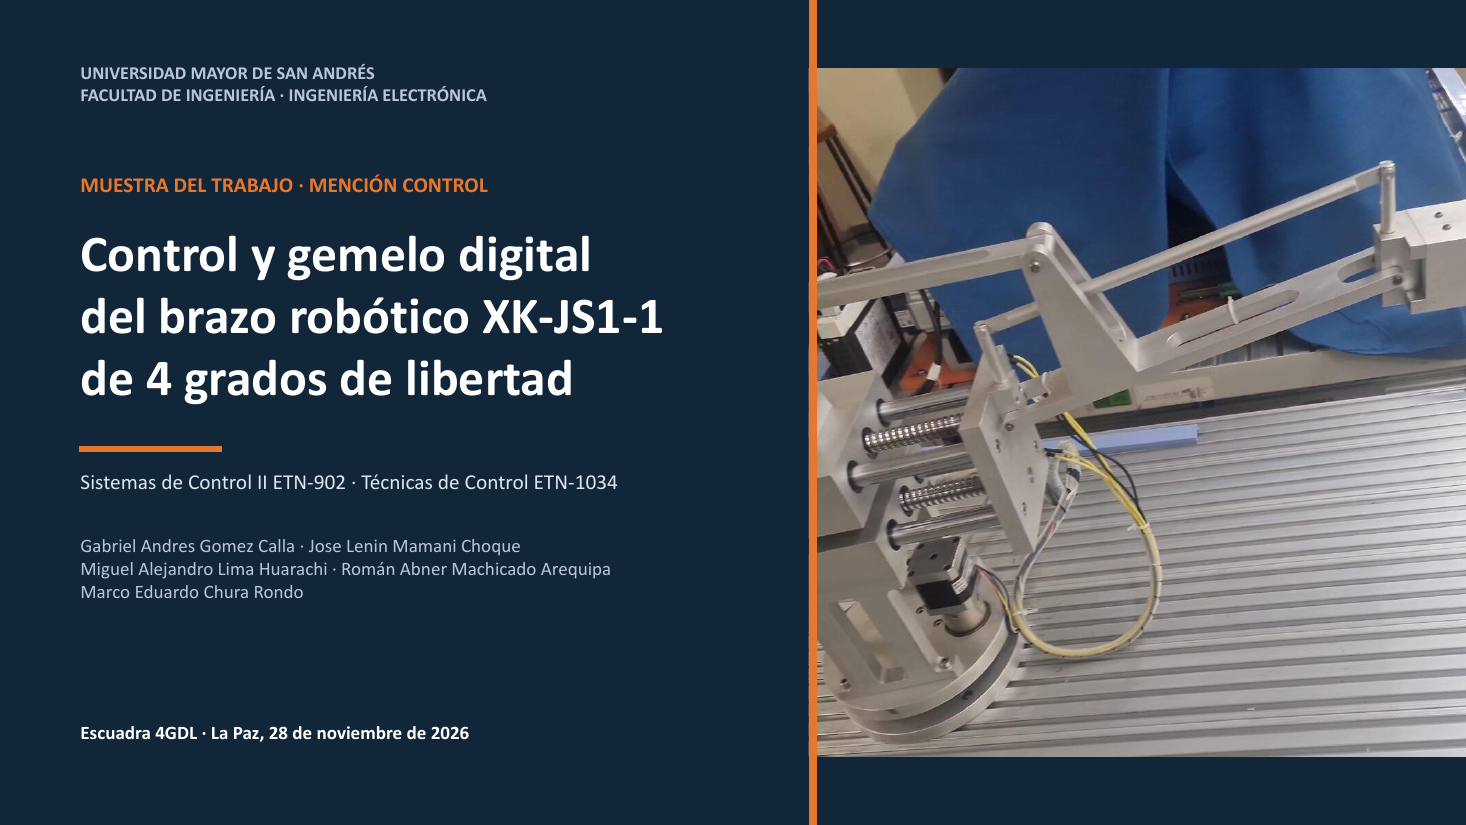
\includegraphics[width=\linewidth]{laminas/l-01.png}\end{center}
\noindent\textbf{Qué muestra.} Presenta el tema, el equipo y las materias del área de control a las que responde el trabajo (ETN-902 y ETN-1034). La foto es la planta real del laboratorio.

\begin{guion}{0:00 -- 0:30 \quad (30 s)}
Buenos días. Somos la Escuadra 4GDL y vamos a mostrar el trabajo hecho este semestre sobre el brazo robótico XK-JS1-1 del laboratorio, visto desde la mención de control: cómo está instrumentado, cómo se modela, qué controladores se pueden diseñar con el hardware que tiene, y el gemelo digital que construimos para supervisarlo y operarlo. Al final haremos una demostración en vivo de la aplicación.
\end{guion}
\clearpage

\section*{Lámina 02 · De una maqueta sin documentación a una planta modelada y supervisada}
\addcontentsline{toc}{subsection}{Lámina 02 · De una maqueta sin documentación a una planta modelada y supervisada}
\begin{center}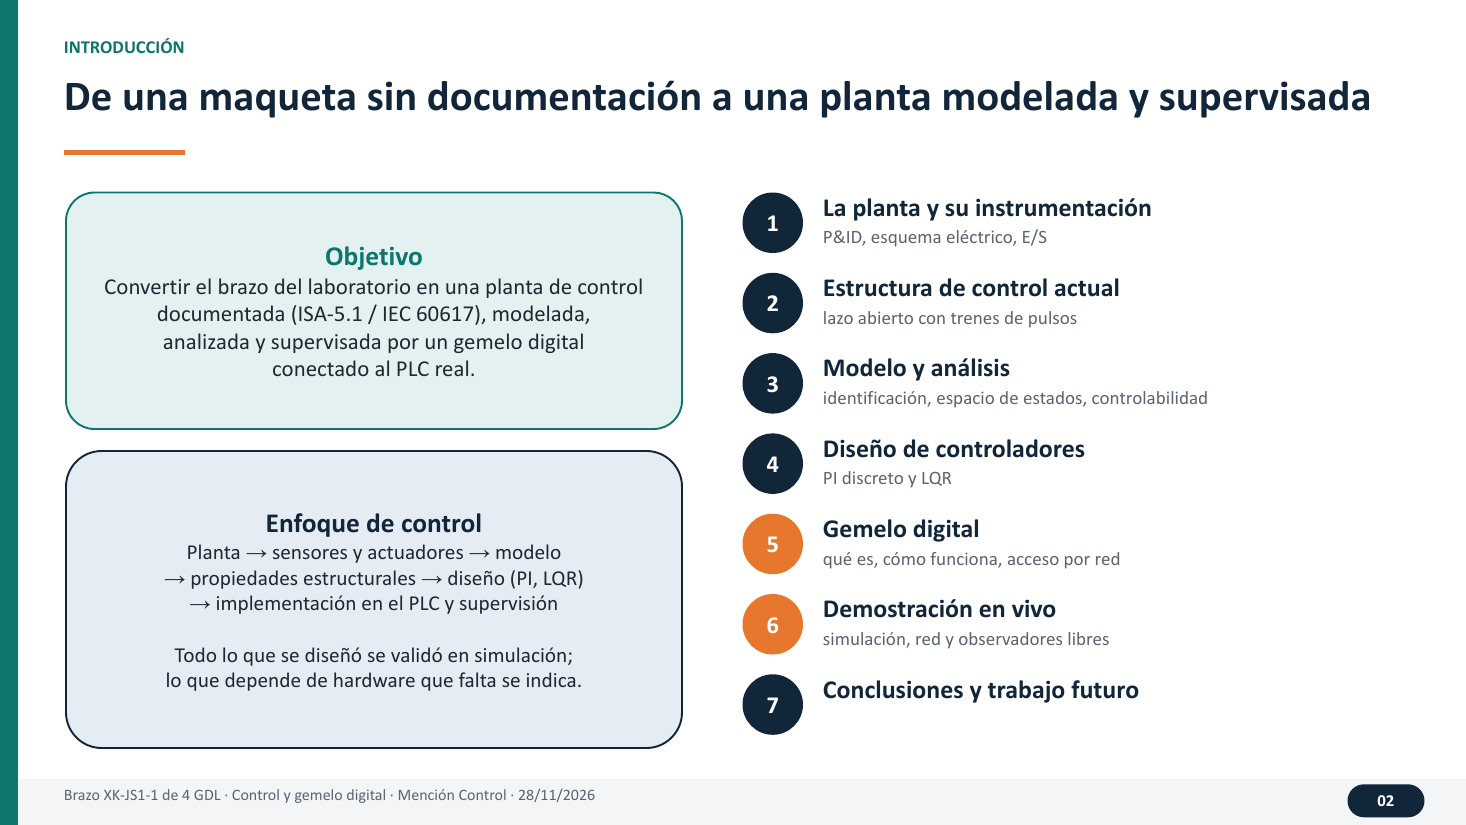
\includegraphics[width=\linewidth]{laminas/l-02.png}\end{center}
\noindent\textbf{Qué muestra.} El objetivo del trabajo y el orden de la exposición. La columna de la derecha sirve de mapa: cada bloque corresponde a una parte del ciclo clásico de un ingeniero de control (planta $\rightarrow$ instrumentación $\rightarrow$ modelo $\rightarrow$ análisis $\rightarrow$ diseño $\rightarrow$ implementación y supervisión).

\begin{guion}{0:30 -- 1:15 \quad (45 s)}
El punto de partida fue una maqueta que funcionaba con un programa heredado, sin planos confiables ni modelo. El objetivo fue convertirla en una planta de control: documentada con normas, modelada, analizada y supervisada por un gemelo digital. La presentación sigue ese mismo orden: primero la planta y su instrumentación, después la estructura de control y el modelo, luego los controladores diseñados, el gemelo digital y, por último, la demostración.
\end{guion}
\clearpage

\section*{Lámina 03 · Brazo XK-JS1-1: tres ejes con motores paso a paso y una garra}
\addcontentsline{toc}{subsection}{Lámina 03 · Brazo XK-JS1-1: tres ejes con motores paso a paso y una garra}
\begin{center}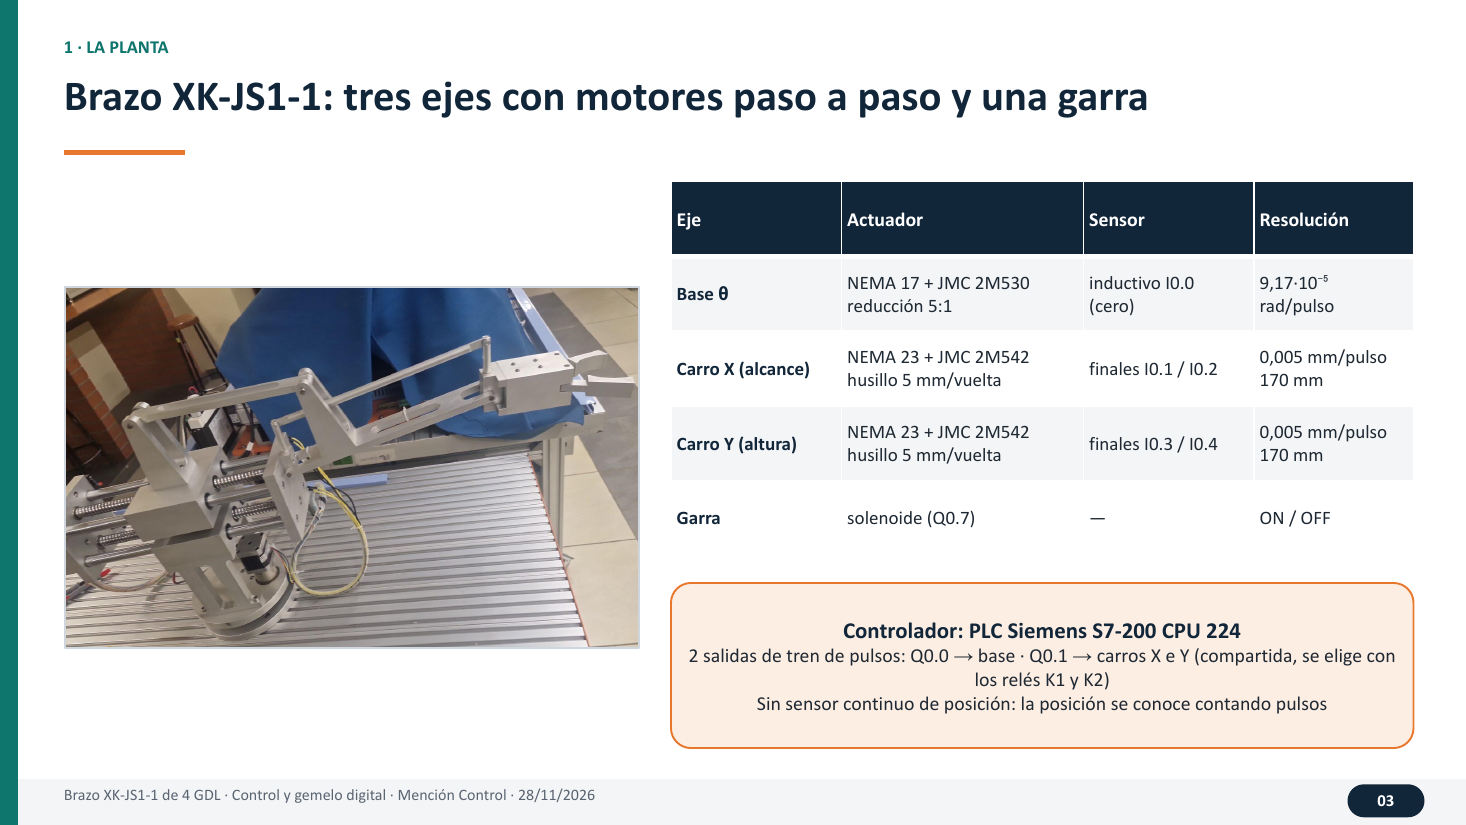
\includegraphics[width=\linewidth]{laminas/l-03.png}\end{center}
\noindent\textbf{Qué muestra.} Los componentes de la planta agrupados por función de control. Lo esencial para el resto de la presentación: (1) los actuadores son motores paso a paso, que se mandan por número de pulsos; (2) el PLC tiene dos generadores de trenes de pulsos (PTO) para tres ejes; (3) todos los sensores son binarios (finales de carrera e inductivo), no hay medición continua de la posición.

\begin{guion}{1:15 -- 2:15 \quad (60 s)}
La planta tiene tres ejes y una garra. La base gira con un motor NEMA 17 y una reducción de 5 a 1; los carros X e Y son husillos de 5 milímetros por vuelta movidos por motores NEMA 23. Los drivers JMC trabajan a 1000 pulsos por vuelta, así que cada pulso son 5 micras en los carros. El controlador es un PLC S7-200 CPU 224, que tiene solo dos salidas de tren de pulsos: Q0.0 para la base y Q0.1 compartida por los dos carros. Los sensores son discretos: finales de carrera en X e Y y un inductivo que marca el cero de la base. No hay ningún sensor continuo de posición, y eso va a condicionar todo el análisis de control.
\end{guion}
\clearpage

\section*{Lámina 04 · P\&ID ISA-5.1: cinco lazos, uno por función}
\addcontentsline{toc}{subsection}{Lámina 04 · P\&ID ISA-5.1: cinco lazos, uno por función}
\begin{center}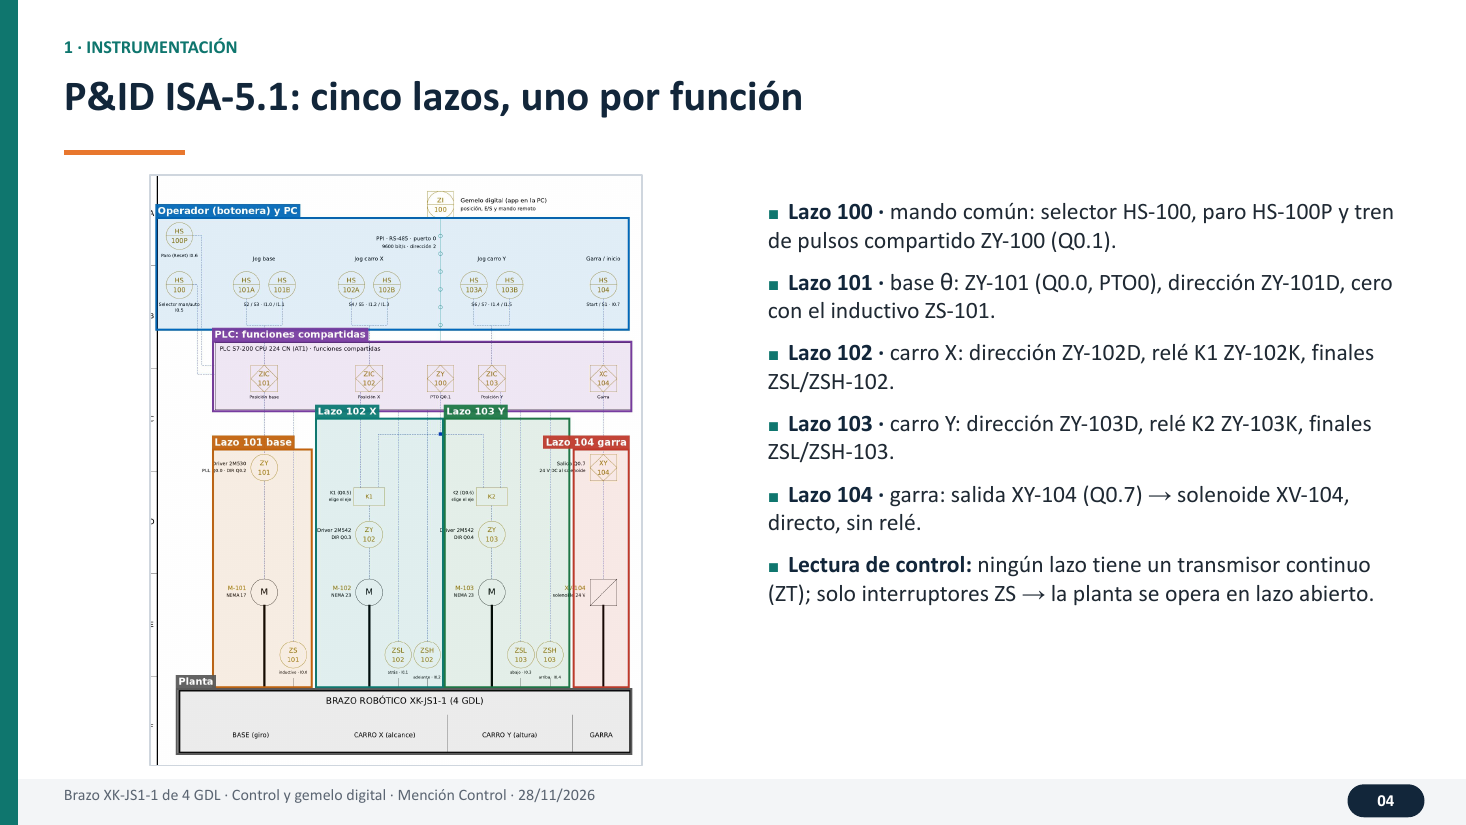
\includegraphics[width=\linewidth]{laminas/l-04.png}\end{center}
\noindent\textbf{Qué muestra.} El diagrama de tuberías e instrumentación (P\&ID) con las zonas coloreadas por lazo. La nomenclatura ISA permite leer cada eje como un lazo de control: ZS = interruptor de posición (final de carrera o inductivo), ZY = relé o convertidor de posición (driver + motor), HS = mando manual, XY/XV = solenoide de la garra. El plano completo (v2.0) está en documentacion/planos\_isa.

\begin{guion}{2:15 -- 2:55 \quad (40 s)}
Para documentarla levantamos de nuevo los planos con la norma ISA 5.1. Cada función es un lazo con su número: el 100 es el mando común y el tren de pulsos compartido de los carros, el 101 la base, el 102 el carro X, el 103 el carro Y y el 104 la garra. En cada lazo los finales de carrera aparecen como interruptores de posición ZS y el driver con su motor como elemento final ZY. La garra se corrigió: el solenoide va directo a la salida Q0.7, sin relé intermedio.
\end{guion}
\clearpage

\section*{Lámina 05 · Esquema eléctrico IEC 60617 y mapa de entradas/salidas}
\addcontentsline{toc}{subsection}{Lámina 05 · Esquema eléctrico IEC 60617 y mapa de entradas/salidas}
\begin{center}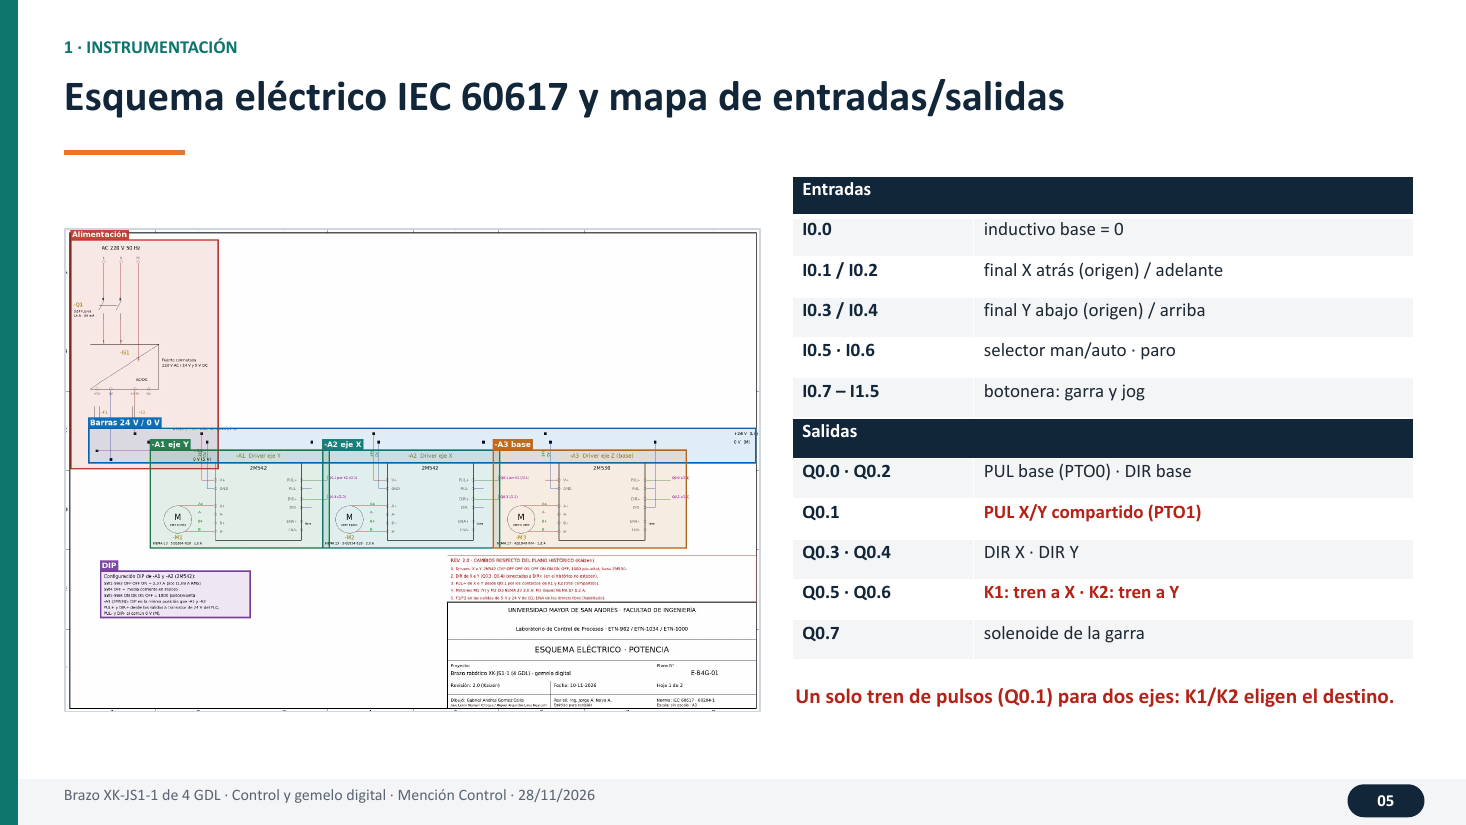
\includegraphics[width=\linewidth]{laminas/l-05.png}\end{center}
\noindent\textbf{Qué muestra.} Plano de potencia (izquierda) y la tabla de E/S resumida. La observación clave es el tren de pulsos compartido: con un solo generador para dos ejes no se pueden mandar velocidades distintas a X e Y al mismo tiempo. El plano de mando (segunda hoja) muestra la botonera y el selector manual/automático.

\begin{guion}{2:55 -- 3:35 \quad (40 s)}
El esquema eléctrico, con norma IEC 60617, muestra el detalle que importa para control: la salida Q0.1 lleva el mismo tren de pulsos a los dos drivers de los carros, y los relés K1 y K2, mandados por Q0.5 y Q0.6, deciden cuál de los dos lo recibe. Si se cierran ambos, X e Y se mueven a la misma velocidad. Esa conexión física es la que después aparece en el modelo como una restricción de controlabilidad.
\end{guion}
\clearpage

\section*{Lámina 06 · Control de posición en lazo abierto con trenes de pulsos}
\addcontentsline{toc}{subsection}{Lámina 06 · Control de posición en lazo abierto con trenes de pulsos}
\begin{center}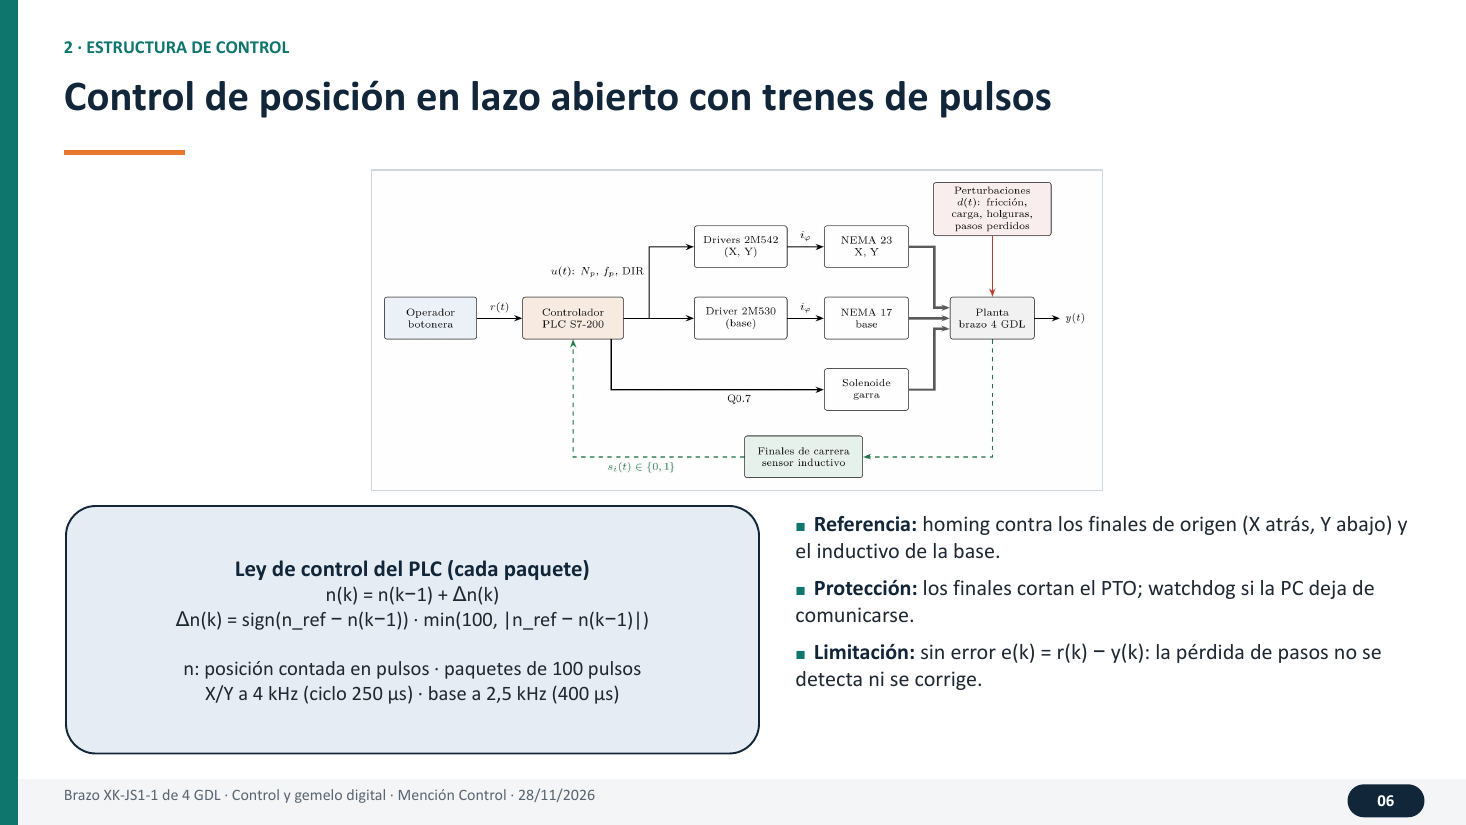
\includegraphics[width=\linewidth]{laminas/l-06.png}\end{center}
\noindent\textbf{Qué muestra.} Diagrama de bloques de la planta: referencia $\rightarrow$ PLC $\rightarrow$ drivers $\rightarrow$ motores paso a paso $\rightarrow$ mecanismo. La realimentación solo existe de forma discreta (finales de carrera e inductivo), que sirven para el homing y para cortar el tren de pulsos en los extremos, pero no para corregir la posición durante el movimiento. La ecuación de diferencias es la que implementa el programa brazo\_gemelo del PLC.

\begin{guion}{3:35 -- 4:35 \quad (60 s)}
Con esa instrumentación, el control que hace hoy el PLC es de posición en lazo abierto. No hay una señal de error entre la referencia y la salida, porque no se mide la salida. El PLC recibe un destino, calcula cuántos pulsos faltan y los envía en paquetes de 100; la posición es la cuenta de pulsos. Esto es una ecuación de diferencias de paso fijo, exacta mientras el motor no pierda pasos. La referencia absoluta la da el homing: los carros van a sus finales de carrera de origen y la cuenta se pone en cero. Las perturbaciones, como fricción, carga o pérdida de pasos, no se detectan: esa es la principal limitación.
\end{guion}
\clearpage

\section*{Lámina 07 · Modelo identificado: integrador con tiempo muerto por eje}
\addcontentsline{toc}{subsection}{Lámina 07 · Modelo identificado: integrador con tiempo muerto por eje}
\begin{center}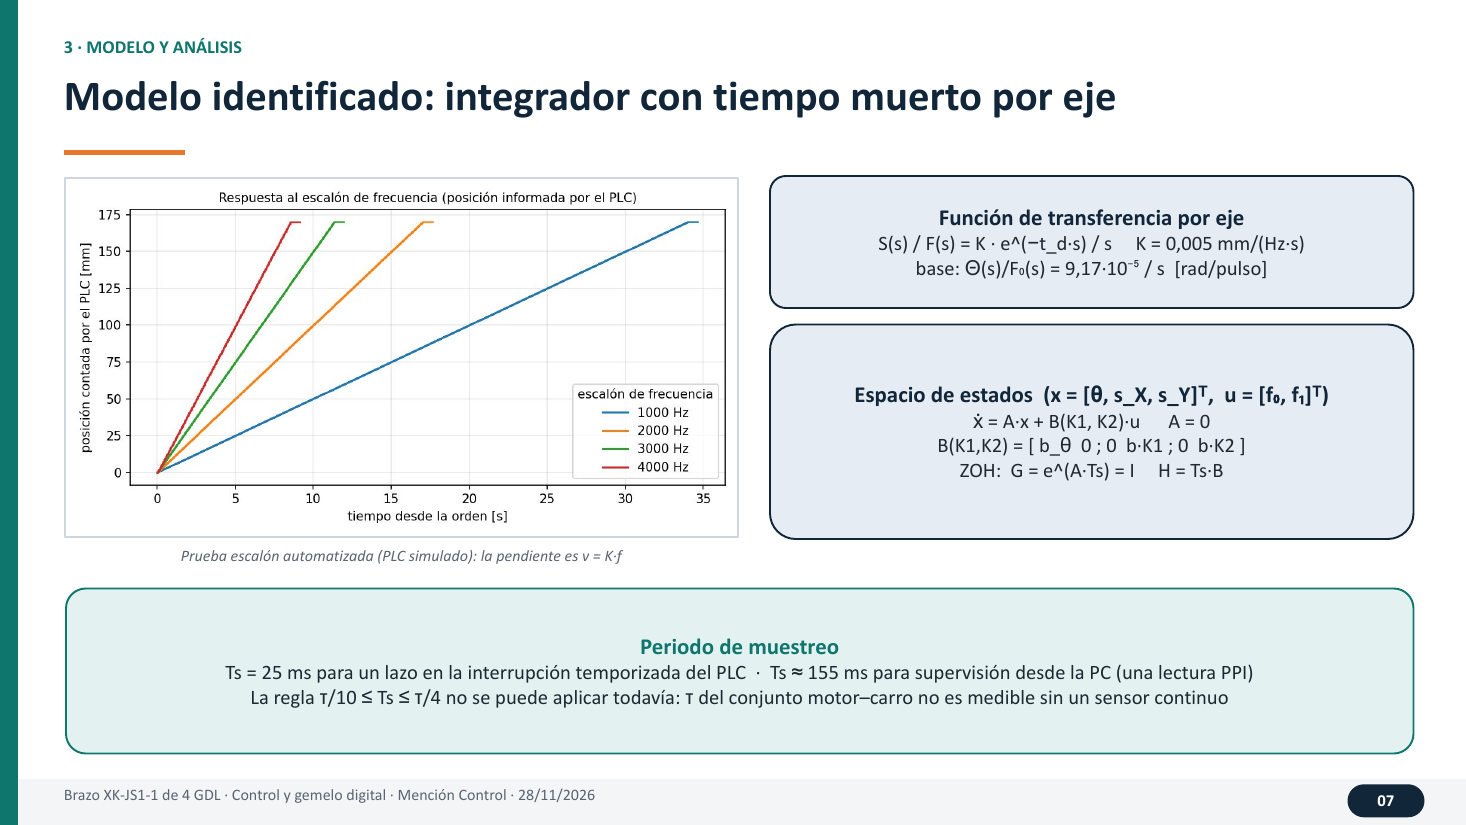
\includegraphics[width=\linewidth]{laminas/l-07.png}\end{center}
\noindent\textbf{Qué muestra.} La identificación por caja negra se hizo con prueba\_escalon.py (laboratorio 4). La figura es una corrida con el PLC simulado de la app: rampas cuya pendiente es la velocidad v = K$\cdot$f. El modelo no tiene la forma K$\cdot$e\^{}(-t\_d s)/($\tau$s+1) porque no hay polo estable observable: el motor paso a paso con su driver se comporta como un integrador de pulsos. El espacio de estados y la discretización ZOH se calcularon con espacio\_estados\_brazo.py/.m (laboratorio 5).

\begin{guion}{4:35 -- 5:35 \quad (60 s)}
Para modelar automatizamos una prueba escalón: el programa lleva el eje a cero, aplica un escalón de frecuencia y registra lo que informa el PLC. Lo que sí se puede medir es el tiempo muerto, que es la latencia de la comunicación más el ciclo del PLC, y la ganancia, que es la velocidad entre la frecuencia. El modelo de cada eje queda como un integrador con tiempo muerto: posición sobre frecuencia igual a K por e a la menos t\_d s, sobre s, con K igual a 5 micras por pulso. En espacio de estados la matriz A es cero y la B depende de qué relé está cerrado. Al discretizar con retención de orden cero, G es la identidad y H es Ts por B. Proponemos 25 milisegundos para un lazo dentro del PLC y unos 155 milisegundos para supervisión desde la PC, que es lo que tarda una lectura por PPI. La constante de tiempo del motor no se puede identificar sin un sensor continuo.
\end{guion}
\clearpage

\section*{Lámina 08 · Controlabilidad y observabilidad: el hardware limita el control}
\addcontentsline{toc}{subsection}{Lámina 08 · Controlabilidad y observabilidad: el hardware limita el control}
\begin{center}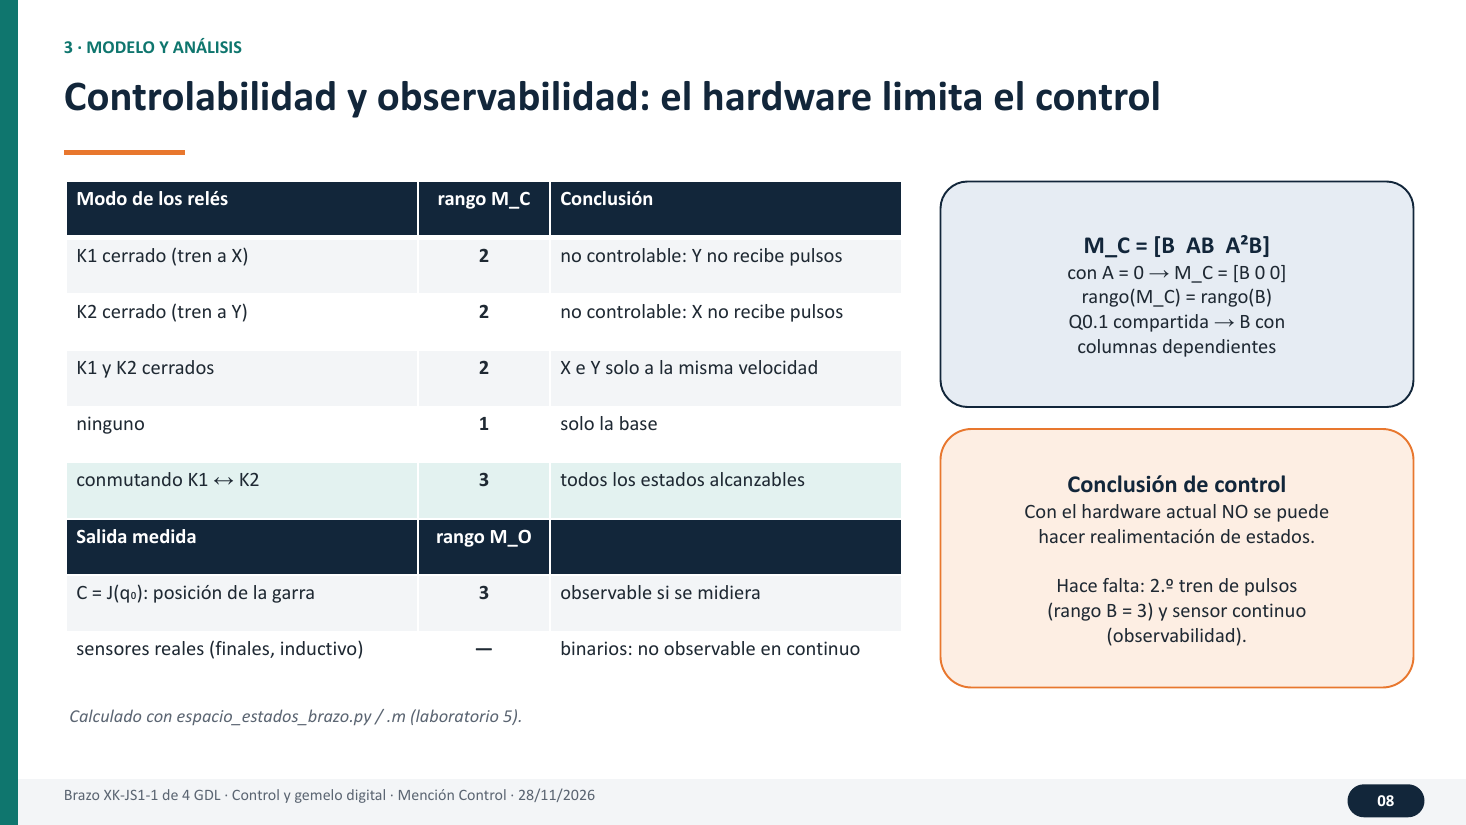
\includegraphics[width=\linewidth]{laminas/l-08.png}\end{center}
\noindent\textbf{Qué muestra.} Resultados de espacio\_estados\_brazo.py (salida\_espacio\_estados.txt, laboratorio 5). Esta lámina conecta el plano eléctrico (Q0.1 compartida) con la teoría: la restricción física aparece como pérdida de rango en B. Es el argumento técnico para las mejoras de hardware propuestas al final.

\begin{guion}{5:35 -- 6:20 \quad (45 s)}
Con el modelo calculamos las matrices de controlabilidad y observabilidad. Como A es cero, el rango de Mc es el rango de B. Con un solo relé cerrado, o con los dos, el rango es 2 de 3: el sistema no es controlable, porque los dos carros comparten el mismo tren de pulsos. Solo conmutando K1 y K2 se alcanzan todos los estados, que es justamente lo que hace el programa: un tramo común y luego el resto del eje más largo. En observabilidad, si se midiera la posición el rango sería 3, pero con sensores binarios no hay una salida lineal: no es observable. Conclusión: con el hardware actual no se puede hacer realimentación de estados; hace falta un segundo tren de pulsos y un sensor continuo.
\end{guion}
\clearpage

\section*{Lámina 09 · PI discreto por asignación de polos (listo para cuando haya sensor)}
\addcontentsline{toc}{subsection}{Lámina 09 · PI discreto por asignación de polos (listo para cuando haya sensor)}
\begin{center}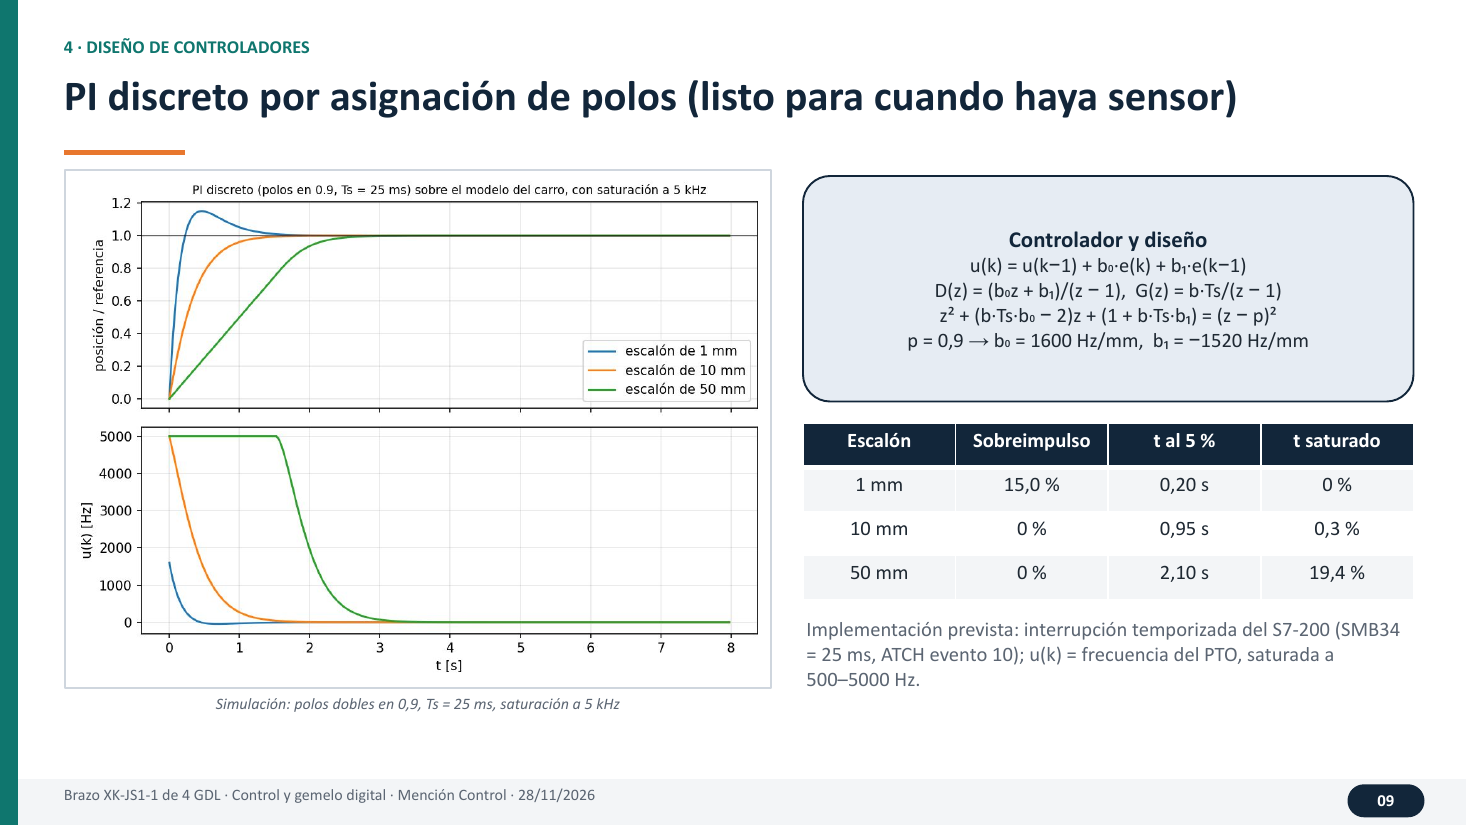
\includegraphics[width=\linewidth]{laminas/l-09.png}\end{center}
\noindent\textbf{Qué muestra.} Diseño del laboratorio 6 (pi\_discreto.py y pi\_discreto.m). La ley u(k) = u(k-1) + b0$\cdot$e(k) + b1$\cdot$e(k-1) se ejecutaría en la interrupción temporizada (SMB34 = 25 ms, ATCH al evento 10), guardando e(k-1) y u(k-1) en memoria V, con u(k) como frecuencia del PTO saturada entre 500 y 5000 Hz. La rutina está escrita (pi\_lazo\_flotante.awl) pero no se cargó en el PLC porque no hay sensor de posición.

\begin{guion}{6:20 -- 7:20 \quad (60 s)}
Aun así diseñamos los controladores para cuando exista realimentación. Primero un PI discreto por eje, pensado para la interrupción temporizada del S7-200 a 25 milisegundos. Con la planta b por Ts sobre z menos 1 y el controlador b0 z más b1 sobre z menos 1, el polinomio característico es de segundo orden. Ubicando un polo doble en 0,9 salen b0 igual a 1600 y b1 igual a menos 1520 hercios por milímetro. La simulación con saturación a 5 kilohercios muestra que para escalones pequeños hay un 15 por ciento de sobreimpulso, que produce el cero del PI, y para escalones grandes el actuador satura, pero no hay sobreimpulso.
\end{guion}
\clearpage

\section*{Lámina 10 · LQR: qué se puede con el hardware actual y con el propuesto}
\addcontentsline{toc}{subsection}{Lámina 10 · LQR: qué se puede con el hardware actual y con el propuesto}
\begin{center}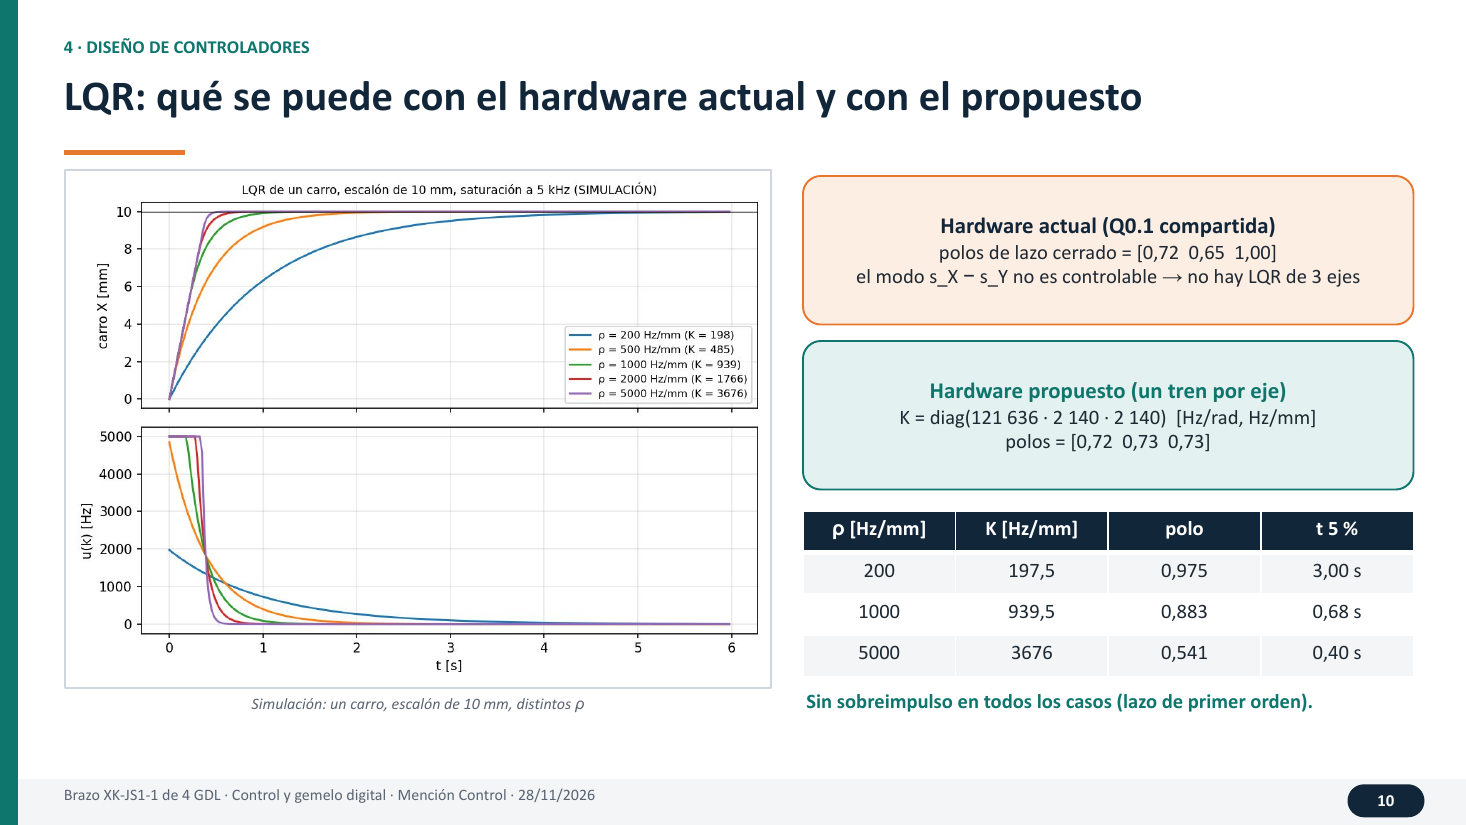
\includegraphics[width=\linewidth]{laminas/l-10.png}\end{center}
\noindent\textbf{Qué muestra.} Resultados de lqr\_brazo.py / lqr\_brazo.m (laboratorio 7, salida\_lqr.txt). Q = diag(1/(1$^\circ$)$^2$, 1/mm$^2$, 1/mm$^2$), R = diag(1/(2500 Hz)$^2$). Con integrador puro y realimentación de estado, el lazo cerrado es de primer orden, sin sobreimpulso. El LQR no se implementó en el PLC porque requiere medir el estado.

\begin{guion}{7:20 -- 8:05 \quad (45 s)}
El segundo diseño es un regulador cuadrático óptimo. Con el hardware actual, cualquier ganancia deja un polo en z igual a 1: el modo diferencia entre los dos carros no es controlable, así que no existe un LQR de tres ejes. Con un tren de pulsos por eje, que es la mejora propuesta, la ganancia es diagonal y los polos quedan entre 0,72 y 0,73. Para un carro solo, variando el peso rho, el lazo es de primer orden y no tiene sobreimpulso: es la ventaja frente al PI. Con rho de 1000 se llega al 5 por ciento en 0,68 segundos.
\end{guion}
\clearpage

\section*{Lámina 11 · Cinemática: de los carros a la posición de la garra}
\addcontentsline{toc}{subsection}{Lámina 11 · Cinemática: de los carros a la posición de la garra}
\begin{center}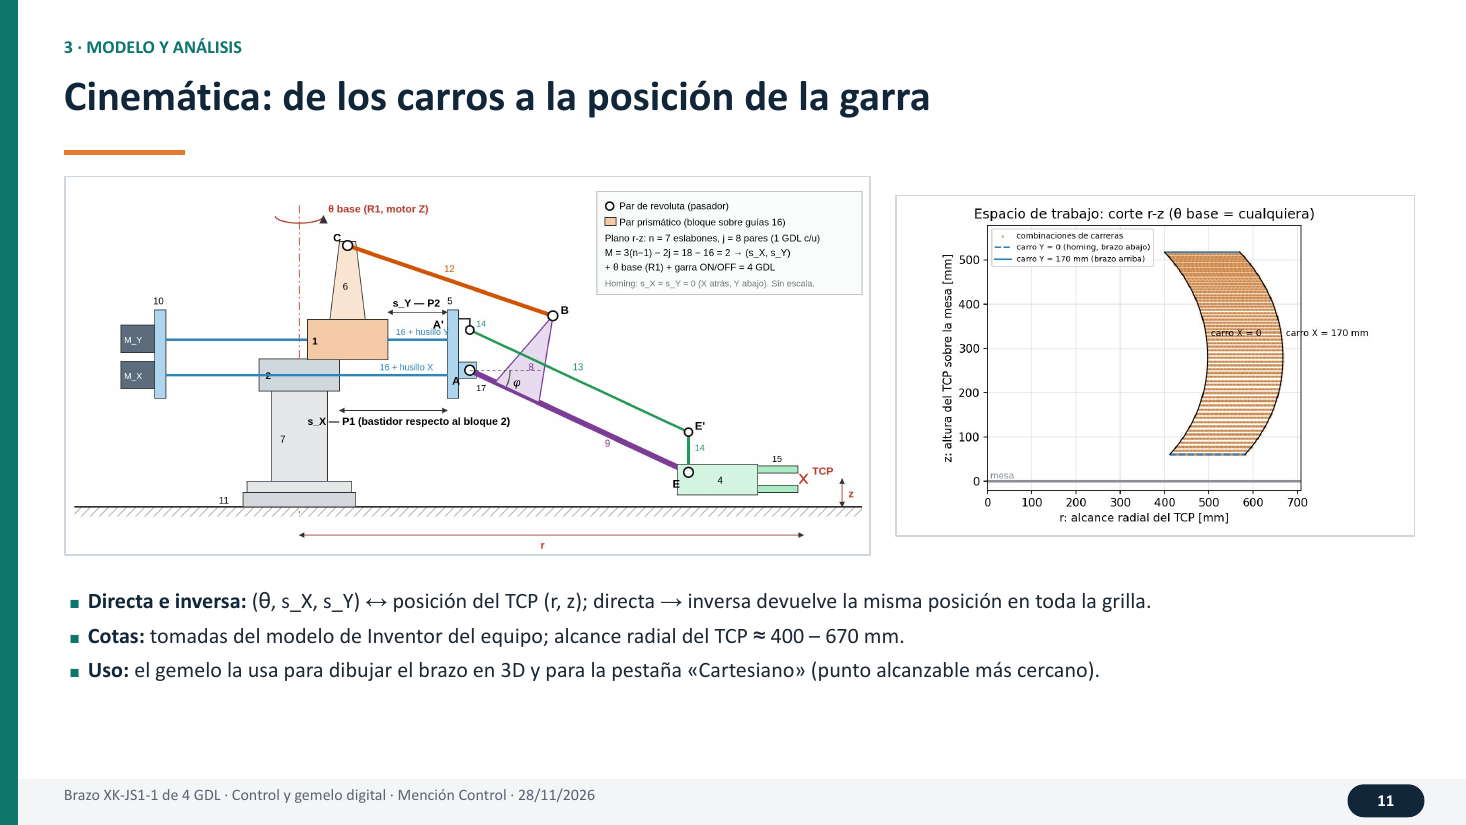
\includegraphics[width=\linewidth]{laminas/l-11.png}\end{center}
\noindent\textbf{Qué muestra.} Esquema cinemático (izquierda) y el corte r--z del espacio de trabajo (derecha). La cinemática directa lleva ($\theta$, s\_X, s\_Y) a la posición del TCP; la inversa resuelve el problema contrario y se verificó que directa seguida de inversa devuelve la misma posición en toda la grilla. El jacobiano relaciona velocidades de los carros con velocidades de la garra (manual técnico, capítulo 8).

\begin{guion}{8:05 -- 8:35 \quad (30 s)}
El último modelo es el geométrico. El brazo es un mecanismo de barras: las posiciones de los carros X e Y y el ángulo de la base determinan dónde está la garra. Obtuvimos la cinemática directa, la inversa y el jacobiano, con las cotas del modelo de Inventor del equipo. El espacio de trabajo es una corona entre unos 400 y 670 milímetros de alcance. Este modelo es el que usa el gemelo digital para dibujar el brazo y para convertir un punto cartesiano en posiciones de los carros.
\end{guion}
\clearpage

\section*{Lámina 12 · Gemelo digital: una réplica virtual sincronizada con el PLC real}
\addcontentsline{toc}{subsection}{Lámina 12 · Gemelo digital: una réplica virtual sincronizada con el PLC real}
\begin{center}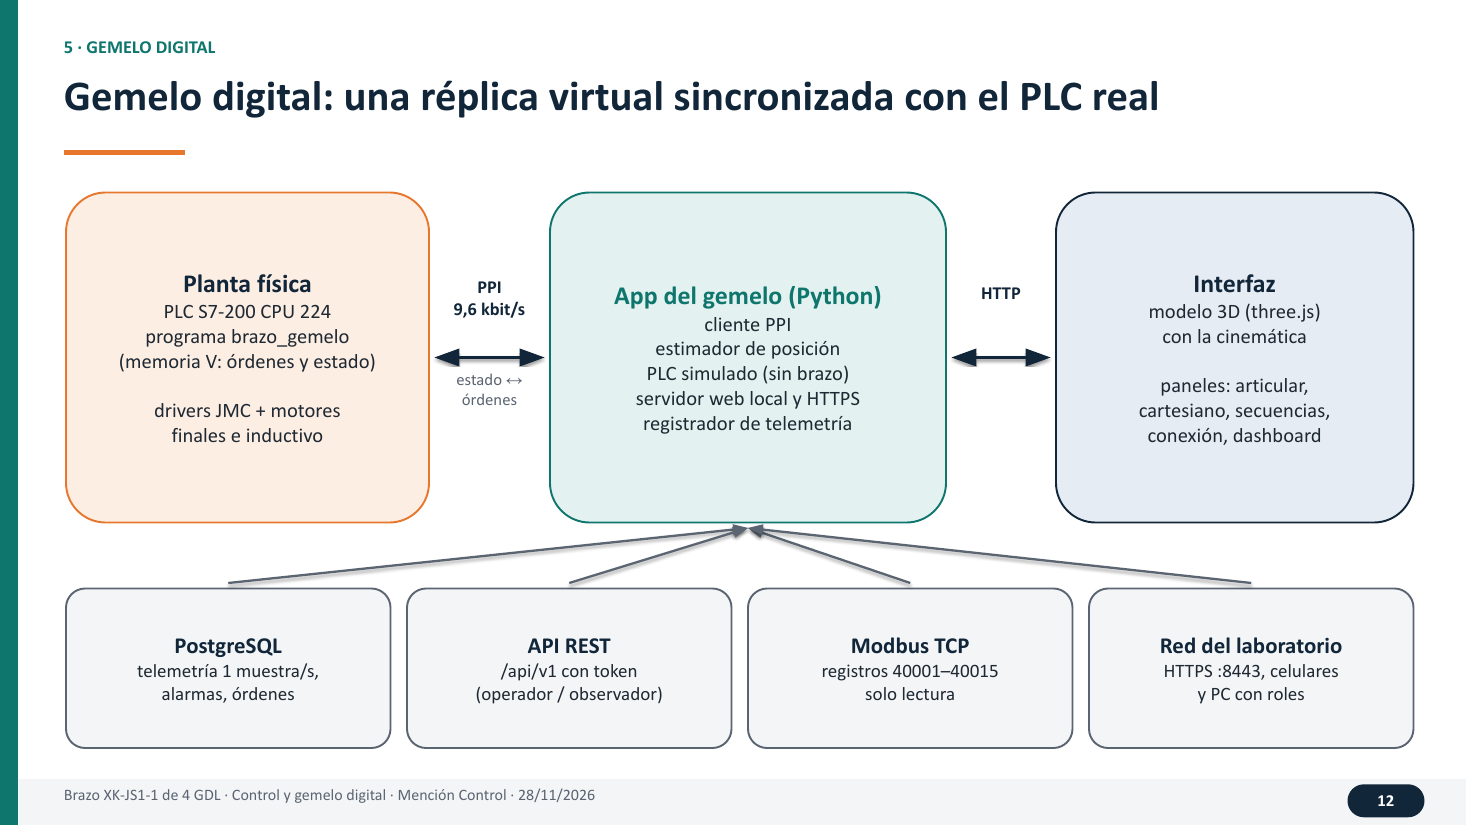
\includegraphics[width=\linewidth]{laminas/l-12.png}\end{center}
\noindent\textbf{Qué muestra.} Arquitectura del gemelo. Planta física $\leftrightarrow$ protocolo PPI (RS-485, 9,6 kbit/s, cable USB-PPI) $\leftrightarrow$ aplicación en Python (cliente PPI, estimador de posición, PLC simulado, servidor web, registrador de telemetría) $\leftrightarrow$ interfaz web con el modelo 3D (three.js). La misma app corre en Linux y Windows, sin internet. Se eligió una app propia en lugar de Simulink porque, además de simular, debía conectarse al PLC y servir de interfaz de operación.

\begin{guion}{8:35 -- 9:35 \quad (60 s)}
Con todo eso construimos el gemelo digital: una réplica virtual del brazo que está sincronizada con la planta real. Del lado físico está el PLC con su programa, los drivers y los motores. La aplicación, escrita en Python, se conecta al puerto del PLC con un cable USB-PPI a 9,6 kilobits por segundo, lee su memoria, calcula la posición y la muestra en un modelo 3D con la cinemática que acabamos de ver. Funciona en ambos sentidos: también manda órdenes al PLC. Y alrededor tiene los servicios de supervisión: la base de datos PostgreSQL con la telemetría, una API REST, una pasarela Modbus TCP y el acceso por la red del laboratorio para celulares y otras computadoras.
\end{guion}
\clearpage

\section*{Lámina 13 · Cómo funciona: el ciclo de lectura, cálculo y mando}
\addcontentsline{toc}{subsection}{Lámina 13 · Cómo funciona: el ciclo de lectura, cálculo y mando}
\begin{center}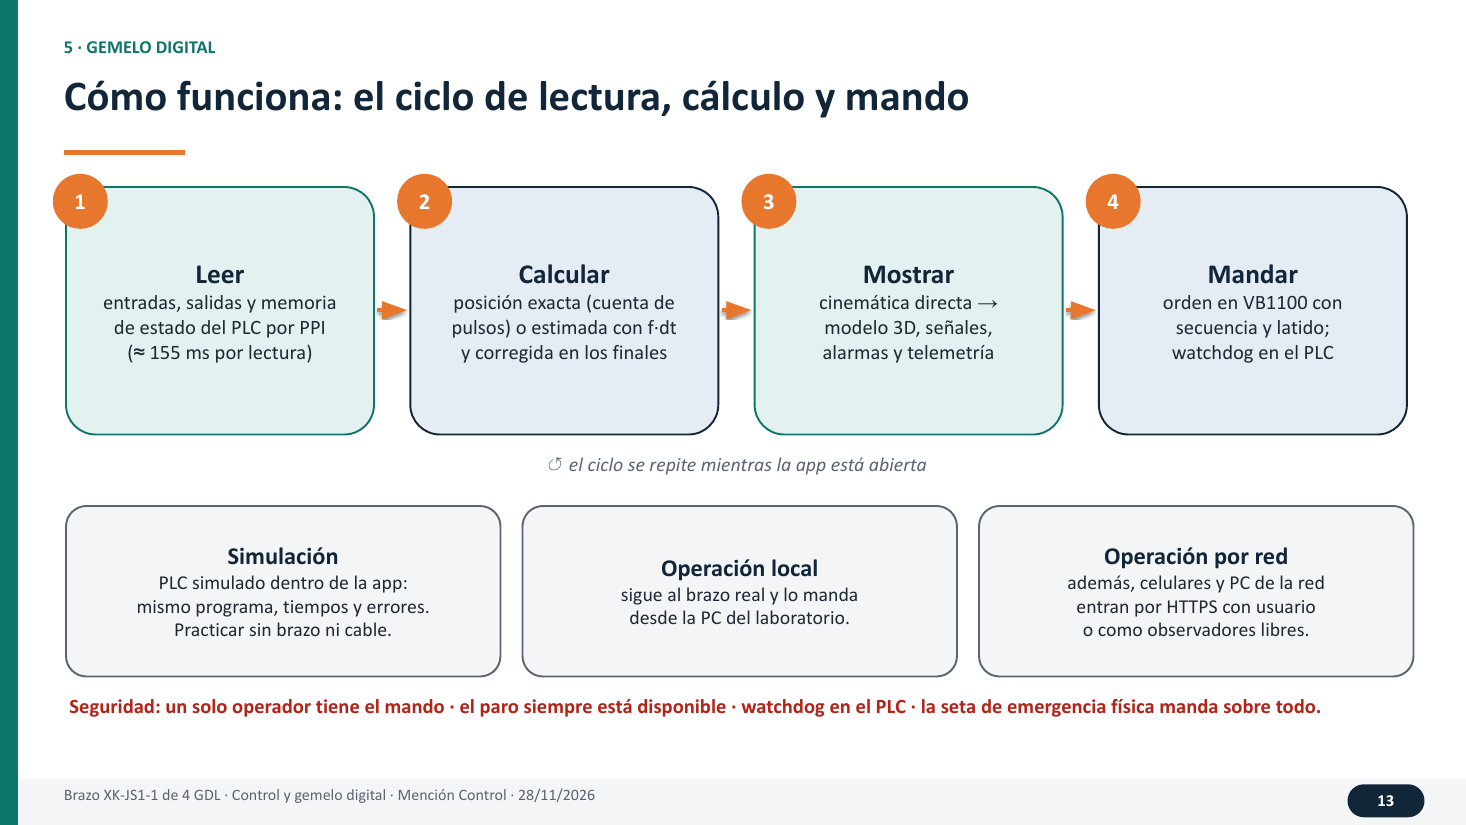
\includegraphics[width=\linewidth]{laminas/l-13.png}\end{center}
\noindent\textbf{Qué muestra.} El ciclo del gemelo. La interfaz PC--PLC es un bloque de memoria V: VB1100 (orden), VB1101 (secuencia), VW1102 (latido), VD1104--VD1112 (destino en pulsos) y, de vuelta, VB1120--VB1141 (estado, posición, entradas, salidas y firma del programa). El estimador se validó contra el programa original con pruebas\_estimador.py (error máximo 1,35 mm en 170 mm, 99,2 \%).

\begin{guion}{9:35 -- 10:35 \quad (60 s)}
El funcionamiento es un ciclo. Primero la app lee del PLC las entradas, las salidas y la memoria de estado; una lectura tarda unos 155 milisegundos. Segundo, calcula la posición: con nuestro programa brazo\_gemelo el PLC cuenta los pulsos y la posición es exacta al pulso; con el programa original, que no cuenta, la app la estima integrando la frecuencia de los trenes y la corrige en los finales de carrera, con un error máximo de 1,35 milímetros. Tercero, aplica la cinemática y mueve el modelo 3D. Cuarto, si el operador da una orden, la escribe en la memoria V: homing, mover, paro o garra, con un número de secuencia y un latido; si la PC deja de responder, el watchdog del PLC detiene el brazo. La app tiene tres modos: simulación, operación local y operación por red.
\end{guion}
\clearpage

\section*{Lámina 14 · Acceso por red: operadores, observadores y observadores libres}
\addcontentsline{toc}{subsection}{Lámina 14 · Acceso por red: operadores, observadores y observadores libres}
\begin{center}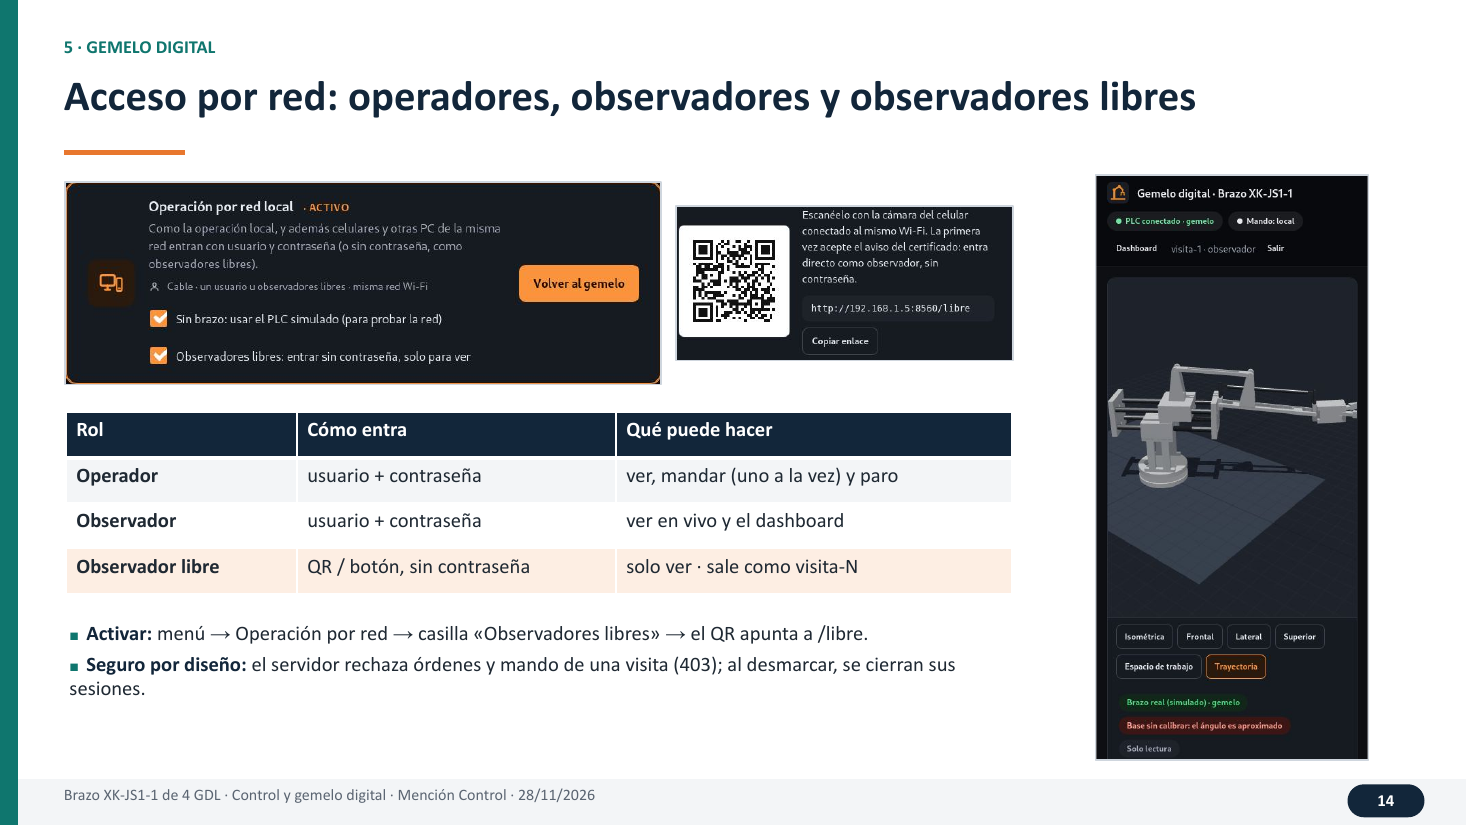
\includegraphics[width=\linewidth]{laminas/l-14.png}\end{center}
\noindent\textbf{Qué muestra.} Roles del acceso por red: operador (usuario y contraseña; ve y manda, uno a la vez), observador con usuario (solo ve) y, desde esta versión, observador libre (sin contraseña, solo ve). La casilla está en el menú, se puede activar también con --observadores-libres, y viene apagada al abrir la app. El servidor valida el rol en cada petición: una visita recibe 403 si intenta mover o tomar el mando. Las contraseñas de los usuarios se guardan con PBKDF2-SHA256 y la conexión va cifrada con un certificado propio.

\begin{guion}{10:35 -- 11:25 \quad (50 s)}
Para clases y demostraciones agregamos los observadores libres. En el modo de operación por red, el menú tiene una casilla nueva: \guillemotleft{}Observadores libres\guillemotright{}. Al marcarla, el código QR de la pantalla lleva directamente a la vista del brazo, sin usuario ni contraseña. Cada persona entra como visita-1, visita-2, etcétera, y ve el brazo en vivo en su celular. Es solo lectura: el servidor rechaza cualquier orden o pedido de mando de una visita, y al desmarcar la casilla se cierran todas esas sesiones. Para mandar el brazo sigue haciendo falta un usuario operador con contraseña.
\end{guion}
\clearpage

\section*{Lámina 15 · Supervisión: telemetría, indicadores e integración industrial}
\addcontentsline{toc}{subsection}{Lámina 15 · Supervisión: telemetría, indicadores e integración industrial}
\begin{center}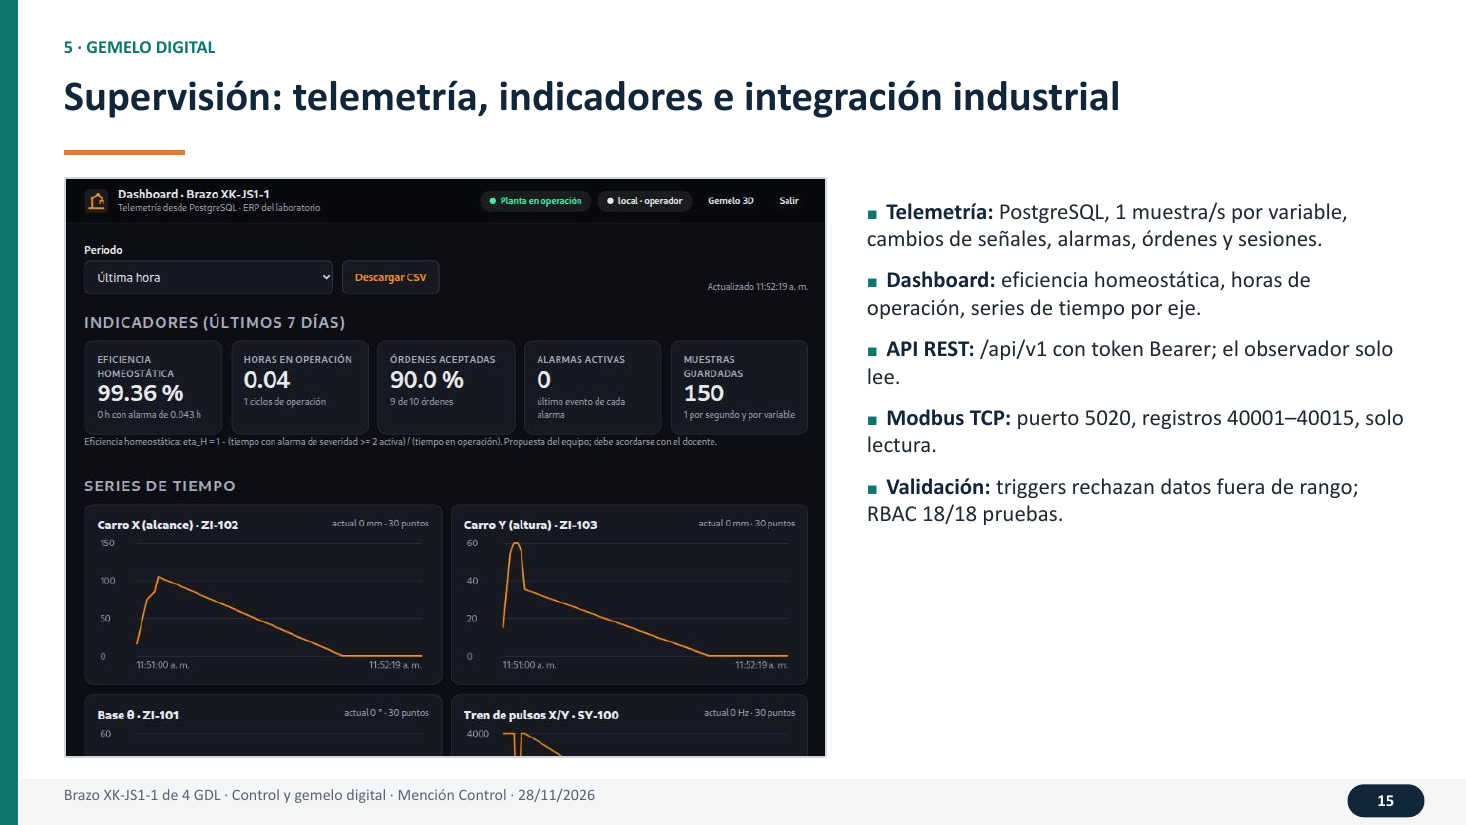
\includegraphics[width=\linewidth]{laminas/l-15.png}\end{center}
\noindent\textbf{Qué muestra.} El dashboard (botón \guillemotleft{}Dashboard\guillemotright{} de la app) lee de PostgreSQL a través de la API. La base tiene triggers que rechazan datos fuera de rango y generan alarmas (laboratorio 5). La pasarela Modbus TCP publica el estado en los registros 40001--40015, solo lectura (laboratorio 8). El certificado RBAC del laboratorio 7 documenta las 18 pruebas de permisos por rol.

\begin{guion}{11:25 -- 11:55 \quad (30 s)}
Todo lo que pasa queda registrado. La app guarda una muestra por segundo de cada variable en PostgreSQL, además de las alarmas, las órdenes y los ingresos. El dashboard muestra indicadores, como la eficiencia homeostática, y las series de tiempo de cada eje. Otros sistemas pueden leer esos datos por la API REST con token o por Modbus TCP, como lo haría un SCADA. Las pruebas de control de acceso por roles pasaron 18 de 18.
\end{guion}
\clearpage

\section*{Lámina 16 · Demostración: la app del gemelo en funcionamiento}
\addcontentsline{toc}{subsection}{Lámina 16 · Demostración: la app del gemelo en funcionamiento}
\begin{center}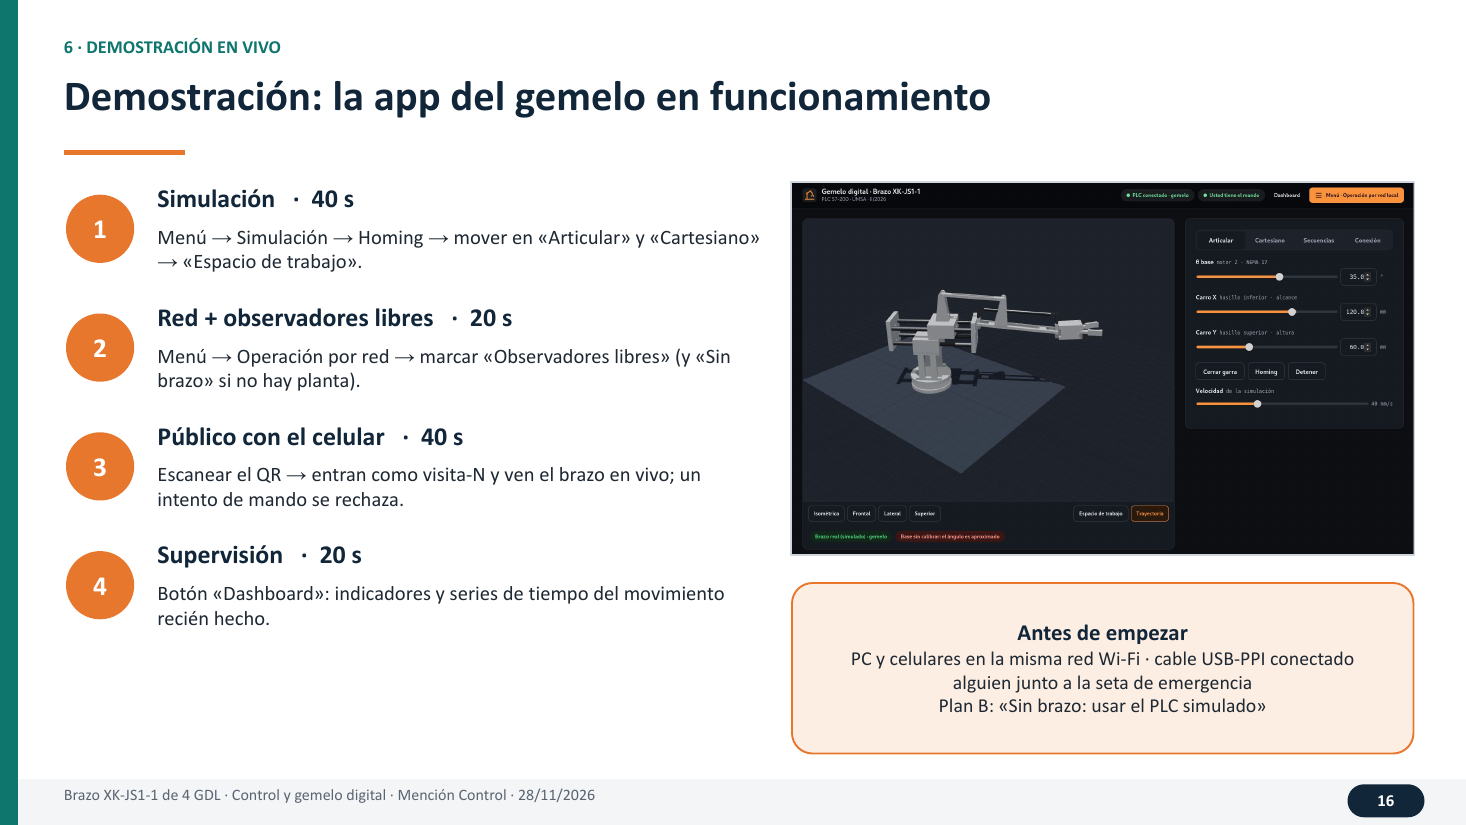
\includegraphics[width=\linewidth]{laminas/l-16.png}\end{center}
\noindent\textbf{Qué muestra.} Guion de la demostración ($\approx$ 2 min). Antes de la presentación: abrir la app, comprobar que la PC y los celulares están en la misma red Wi-Fi y, si se usa el brazo real, que el cable USB-PPI está conectado y alguien está junto a la seta de emergencia. Plan B: casilla \guillemotleft{}Sin brazo: usar el PLC simulado\guillemotright{}.

\begin{guion}{11:55 -- 13:55 \quad (120 s)}
Ahora pasamos a la demostración. Abrimos la app: aparece el menú con los tres modos. [Paso 1] Entramos en simulación, hacemos homing y movemos los ejes desde la pestaña articular; luego en cartesiano elegimos un punto y el gemelo propone el alcanzable más cercano. [Paso 2] Volvemos al menú, elegimos operación por red y marcamos observadores libres. [Paso 3] Les pedimos que escaneen el QR con el celular conectado a la red del laboratorio: van a entrar como visitas y verán el brazo moverse en vivo. Si alguien toca un botón de mando, el servidor lo rechaza. [Paso 4] Mostramos el dashboard con la telemetría. Si el brazo y el cable están conectados, hacemos lo mismo con la planta real; si no, con la casilla \guillemotleft{}sin brazo\guillemotright{} usamos el PLC simulado.
\end{guion}
\clearpage

\section*{Lámina 17 · Resultados, limitaciones y trabajo futuro}
\addcontentsline{toc}{subsection}{Lámina 17 · Resultados, limitaciones y trabajo futuro}
\begin{center}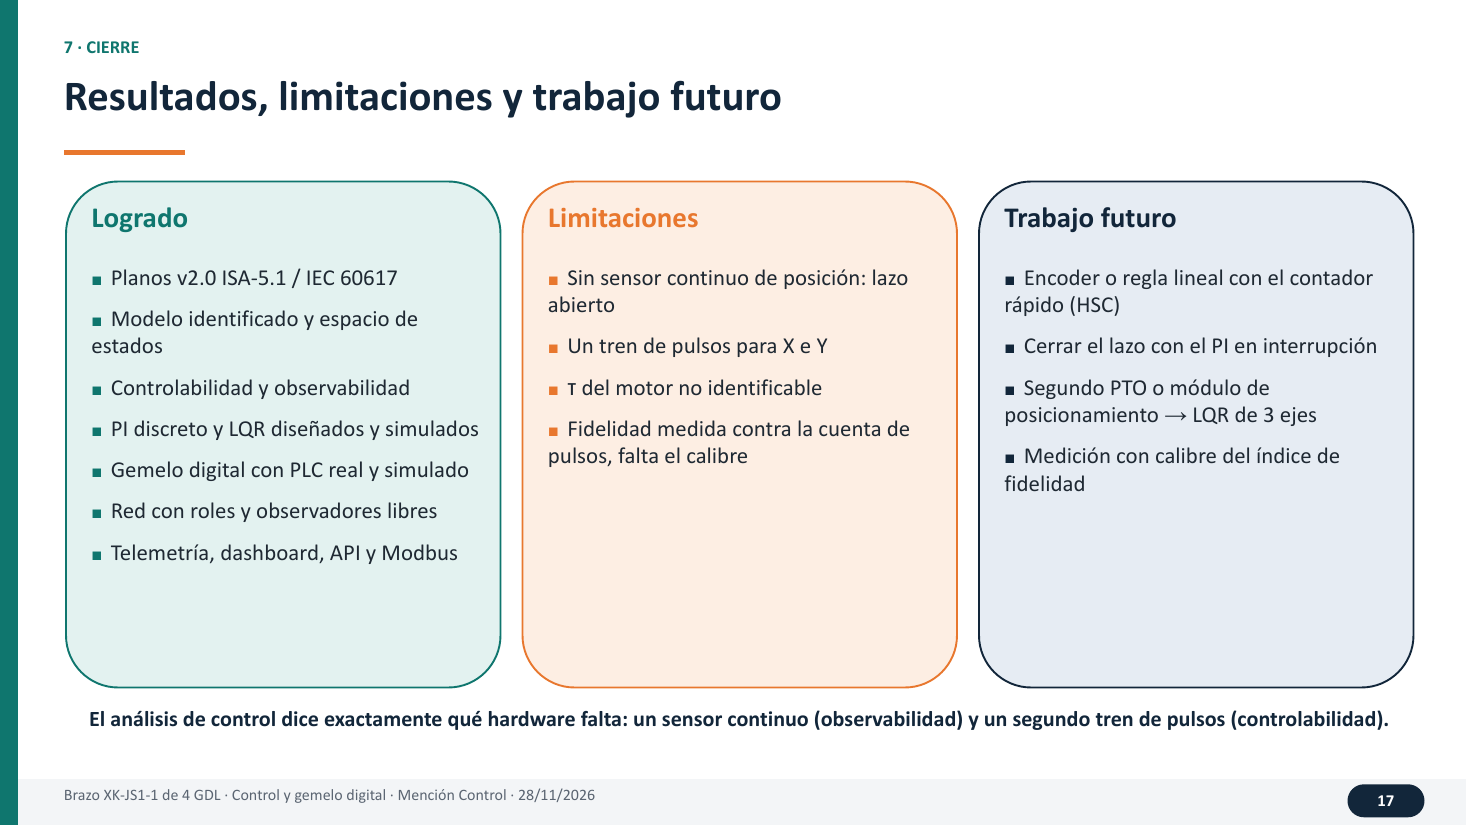
\includegraphics[width=\linewidth]{laminas/l-17.png}\end{center}
\noindent\textbf{Qué muestra.} Resumen de lo logrado, de lo que limita el control y de los pasos siguientes. Las mejoras propuestas salen directamente del análisis de controlabilidad y observabilidad: un sensor continuo hace la planta observable y un segundo tren de pulsos hace que B tenga rango 3.

\begin{guion}{13:55 -- 14:40 \quad (45 s)}
Para cerrar. Logramos documentar la planta con normas, modelarla, analizar sus propiedades estructurales y diseñar dos controladores, y construimos un gemelo digital que funciona con la planta real y en simulación, con supervisión y acceso por red. La principal conclusión de control es que el hardware actual limita la planta a lazo abierto: no hay sensor continuo y dos ejes comparten un tren de pulsos. Las mejoras concretas son un encoder o regla lineal leído con el contador rápido del PLC, para cerrar el lazo con el PI que ya está diseñado, y un segundo generador de pulsos, para el LQR de tres ejes.
\end{guion}
\clearpage

\section*{Lámina 18 · Gracias $\cdot$ Preguntas}
\addcontentsline{toc}{subsection}{Lámina 18 · Gracias $\cdot$ Preguntas}
\begin{center}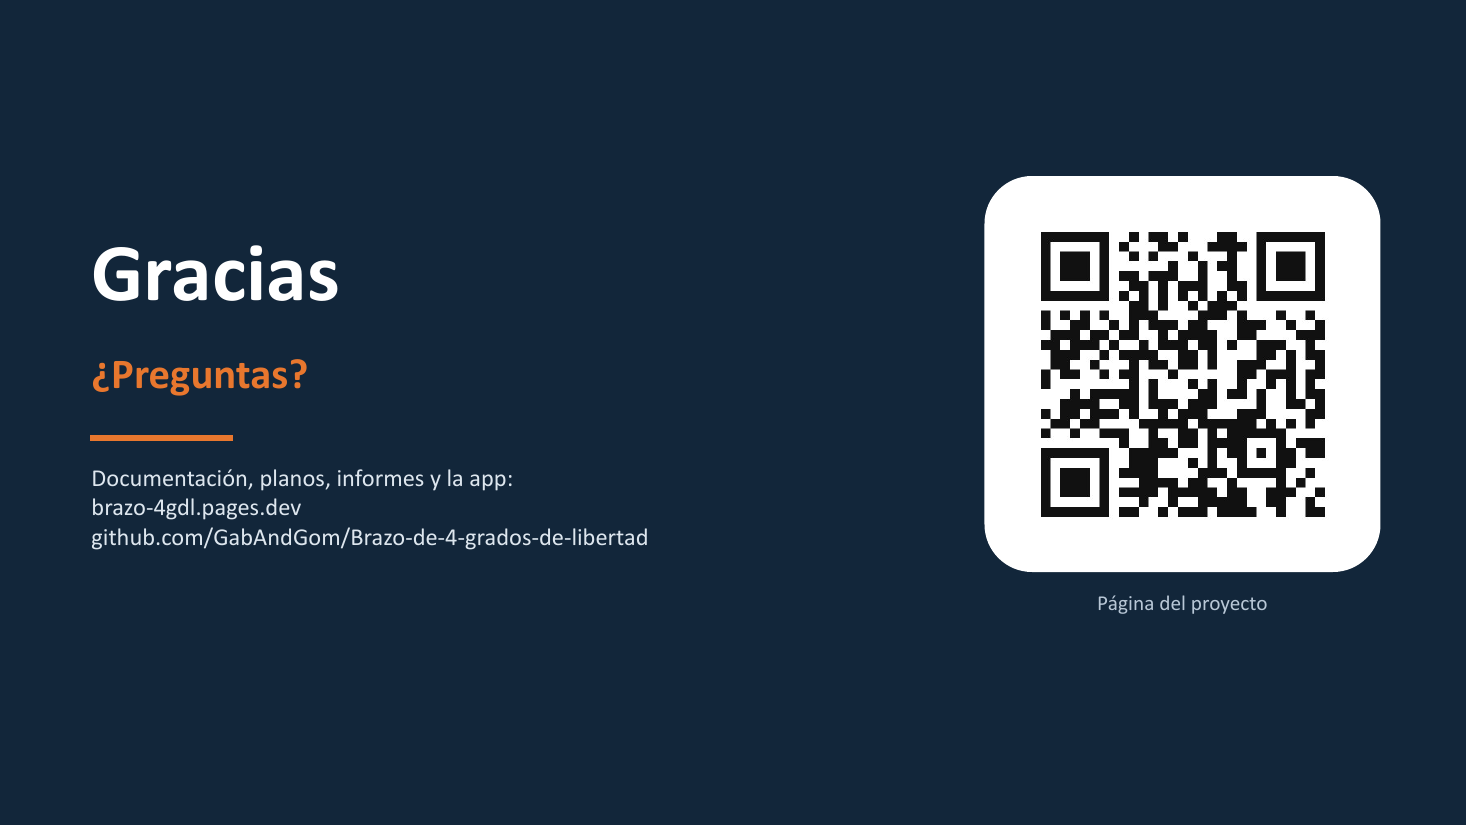
\includegraphics[width=\linewidth]{laminas/l-18.png}\end{center}
\noindent\textbf{Qué muestra.} Cierre con el enlace a la página pública del proyecto y al repositorio.

\begin{guion}{14:40 -- 14:50 \quad (10 s)}
Gracias por su atención. En la página del proyecto, que pueden abrir con este QR, están los planos, los informes, los manuales y la app. Quedamos atentos a sus preguntas.
\end{guion}
\clearpage

\section{El gemelo digital en detalle}
\subsection{Qué es}
Un gemelo digital es una réplica virtual de un sistema físico que se mantiene sincronizada con él: recibe
continuamente los datos de la planta, los representa con un modelo y puede devolverle órdenes. En este proyecto
el gemelo es una aplicación propia en Python, que corre en Linux y Windows sin internet, y una interfaz web con
el modelo 3D del brazo (three.js) construido con la cinemática y las cotas del modelo de Inventor del equipo.
Se eligió una aplicación propia en lugar de Simulink porque, además de simular, debía conectarse al PLC real y
servir de interfaz de operación.

\subsection{Partes de la aplicación}
\begin{center}\small
\begin{tabularx}{\linewidth}{>{\raggedright}p{4.2cm} X}
\toprule
\textbf{Parte} & \textbf{Función}\\
\midrule
Cliente PPI (\codigo{ppi.py}, \codigo{serie.py}) & habla con el PLC S7-200 por su puerto 0 (RS-485) con el cable USB-PPI, a 9,6~kbit/s; lee y escribe la memoria V, las entradas y las salidas\\
Brazo (\codigo{brazo.py}) & reconoce el programa cargado en el PLC (perfil), calcula la posición, valida las órdenes y maneja el mando exclusivo\\
Estimador & con el programa original del PLC, que no cuenta pulsos, estima la posición integrando la frecuencia de los trenes ($f\cdot dt$) y la corrige en los finales de carrera; error máximo 1,35~mm\\
PLC simulado & reproduce el programa \codigo{brazo\_gemelo} (pasos, tiempos y códigos de error) para usar todo sin hardware\\
Servidor (\codigo{gemelo\_brazo.py}) & sirve la interfaz en esta PC (\codigo{localhost:8050}) y, en el modo red, por HTTPS en el puerto 8443; usuarios, roles y observadores libres (\codigo{acceso.py})\\
Telemetría (\codigo{telemetria.py}) & CSV por sesión y PostgreSQL: 1 muestra/s por variable, señales, alarmas, órdenes e ingresos\\
API y Modbus (\codigo{api\_erp.py}, \codigo{modbus.py}) & API REST \codigo{/api/v1} con token y pasarela Modbus TCP de solo lectura (registros 40001--40015)\\
Interfaz (\codigo{ui/}) & modelo 3D, paneles Articular, Cartesiano, Secuencias y Conexión, y el dashboard\\
\bottomrule
\end{tabularx}
\end{center}

\subsection{Interfaz con el PLC (programa \codigo{brazo\_gemelo})}
La PC y el PLC se comunican por un bloque de memoria V. La PC escribe la orden y el PLC devuelve su estado:
\begin{center}\small
\begin{tabular}{l l l}
\toprule
\textbf{Dirección} & \textbf{Quién escribe} & \textbf{Contenido}\\
\midrule
VB1100 & PC & orden: 1 homing, 2 mover, 3 paro, 4 cerrar garra, 5 abrir garra\\
VB1101 & PC & secuencia (aumenta en 1 con cada orden)\\
VW1102 & PC & latido: si deja de cambiar, el watchdog del PLC detiene el brazo\\
VD1104 / VD1108 / VD1112 & PC & destino de la base, X e Y en pulsos (con signo)\\
VB1120 & PLC & estado: 0 reposo, 1 homing, 2 moviendo\\
VB1122 & PLC & banderas: referenciado, remoto, PTO ocupados, posición incierta, watchdog\\
VB1123 & PLC & error: ocupado, fuera de rango, watchdog, sin referencia, paro\\
VD1124 / VD1128 / VD1132 & PLC & posición de la base, X e Y en pulsos\\
VB1138--VB1140 & PLC & copia de IB0, IB1 y QB0; VB1141 = firma 16\#47 del programa\\
\bottomrule
\end{tabular}
\end{center}

\subsection{El ciclo de funcionamiento}
\begin{enumerate}
\item \textbf{Leer.} La app lee del PLC las entradas, las salidas y la memoria de estado. Cada lectura por PPI tarda unos 155~ms; ese es el periodo de supervisión.
\item \textbf{Calcular.} Con \codigo{brazo\_gemelo} la posición es la cuenta de pulsos del PLC, exacta mientras el motor no pierda pasos. Con el programa original, la estima el estimador.
\item \textbf{Mostrar.} La cinemática directa convierte $(\theta, s_X, s_Y)$ en la pose del brazo y el modelo 3D se mueve; se muestran las señales, alarmas y la telemetría.
\item \textbf{Mandar.} Una orden del operador se valida (rol, mando, homing hecho, límites) y se escribe en VB1100 con su secuencia; el PLC la ejecuta y corta los trenes en los finales de carrera.
\end{enumerate}

\subsection{Modos y seguridad}
\begin{itemize}
\item \textbf{Simulación}: PLC simulado; no necesita brazo ni cable.
\item \textbf{Operación local}: sigue al brazo real y lo manda desde la PC del laboratorio; nadie más se conecta.
\item \textbf{Operación por red local}: además, otras PC y celulares de la misma red entran por HTTPS. Roles: operador (ve y manda; uno solo tiene el mando a la vez), observador (solo ve) y observador libre (sin contraseña, solo ve).
\item El paro está siempre disponible; el watchdog del PLC detiene el brazo si la PC deja de comunicarse; la seta de emergencia física manda sobre todo. Las contraseñas se guardan con PBKDF2-SHA256 y sal; tras 5 intentos fallidos una dirección espera 60~s.
\end{itemize}

\subsection{Observadores libres}
Es la novedad de esta versión, pensada para clases y demostraciones con público:
\begin{itemize}
\item Se activa en el menú, en la tarjeta «Operación por red local», con la casilla \textbf{«Observadores libres: entrar sin contraseña, solo para ver»} (o al abrir la app con la opción \codigo{--observadores-libres}). Viene apagada cada vez que se abre la app.
\item Con la casilla marcada, el código QR del menú apunta a \codigo{https://IP:8443/libre}: quien lo escanea entra directo al gemelo como \codigo{visita-1}, \codigo{visita-2}, etc. En la pantalla de ingreso aparece además el botón «Entrar como observador (sin contraseña)».
\item Una visita ve el brazo en vivo y el dashboard, pero el servidor rechaza (código 403) cualquier orden o pedido de mando, y lo anota en el registro.
\item Al desmarcar la casilla, todas las sesiones de visitas se cierran al instante y el enlace \codigo{/libre} deja de funcionar.
\item Para mandar el brazo sigue haciendo falta un usuario operador con contraseña. Con observadores libres activos, la operación por red se puede abrir aunque todavía no haya usuarios creados.
\end{itemize}
Prueba realizada el 28/11/2026 con el PLC simulado: ingreso libre como \codigo{visita-1} (303 al gemelo),
lectura de estado (200), orden de homing y pedido de mando rechazados (403), y tras desactivar la opción la
sesión deja de valer (401) y \codigo{/libre} responde 403.

\clearpage
\section{Guía de la demostración}
\subsection{Antes de la presentación}
\begin{enumerate}
\item Conectar la PC a la red Wi-Fi del laboratorio (la misma que usarán los celulares del público).
\item Si se usará el brazo real: cable USB-PPI al puerto 0 del PLC, selector en remoto (I0.5), tablero energizado y una persona junto a la seta de emergencia. En Linux, si la máquina virtual de Windows XP está abierta, el USB del cable debe estar desmarcado en su menú Dispositivos.
\item Abrir la app: en Linux, menú de aplicaciones $\rightarrow$ \emph{Gemelo digital del brazo} (o \codigo{./iniciar\_gemelo.sh} en la carpeta de la app); en Windows, doble clic en \codigo{Gemelo digital.bat}.
\item Comprobar en el menú, recuadro «Estado», que se detecta el cable (Puertos) o, si no hay brazo, que se usará la casilla «Sin brazo».
\end{enumerate}

\subsection{Durante la demostración (unos 2 minutos)}
\begin{enumerate}
\item \textbf{Simulación (40 s).} Menú $\rightarrow$ Simulación $\rightarrow$ «Abrir». Pulsar «Homing»; en «Articular» mover la base y los carros; en «Cartesiano» elegir un punto (la app propone el alcanzable más cercano); botón «Espacio de trabajo».
\item \textbf{Red y observadores libres (20 s).} Botón «Menú» $\rightarrow$ tarjeta «Operación por red local»: marcar «Sin brazo» si no hay planta, marcar \textbf{«Observadores libres»} y pulsar «Abrir». Volver al menú para ver el QR («Brazo en la red local»).
\item \textbf{Público con el celular (40 s).} Pedir que escaneen el QR. La primera vez el navegador avisa del certificado propio: «Avanzado» $\rightarrow$ «Continuar». Cada uno entra como \codigo{visita-N} y ve el brazo moverse cuando el operador lo mueve desde la PC. Si alguien intenta mandar, aparece el aviso de solo lectura.
\item \textbf{Supervisión (20 s).} Botón «Dashboard»: indicadores y series de tiempo del movimiento recién hecho.
\item Al terminar, desmarcar «Observadores libres» para cerrar las sesiones de las visitas.
\end{enumerate}

\begin{nota}
\textbf{Plan B.} Si el brazo o el cable fallan, todo se puede mostrar con el PLC simulado (casilla «Sin brazo»).
Si los celulares no se conectan (red con aislamiento de clientes), se muestra el ingreso libre desde otra PC o
desde el navegador de la misma PC con la dirección que aparece bajo el QR.
\end{nota}

\subsection{Preguntas probables}
\begin{description}
\item[¿Por qué no hay control en lazo cerrado?] Porque no hay sensor continuo de posición: los finales de carrera y el inductivo son binarios. Sin medir la salida no hay error $e(k)$ que realimentar; la planta no es observable en continuo.
\item[¿Por qué el modelo es un integrador y no un primer orden?] El motor paso a paso con su driver convierte frecuencia en velocidad: la posición es la integral de la frecuencia. La dinámica del conjunto motor--carro, si existe, es de milisegundos y no se puede medir sin un sensor continuo.
\item[¿Qué impide el LQR?] Los carros X e Y comparten el tren de pulsos Q0.1: $B$ tiene rango 2 y el modo $s_X - s_Y$ no es controlable (queda un polo en $z=1$). Con un segundo tren de pulsos sí hay LQR de tres ejes.
\item[¿Qué tan fiel es el gemelo?] Con el programa \codigo{brazo\_gemelo} la posición es exacta al pulso mientras el motor no pierda pasos; con el programa original el estimador tiene un error máximo de 1,35~mm en 170~mm (99,2~\%). Falta la medición independiente con calibre.
\item[¿Es seguro dejar entrar a cualquiera?] El observador libre solo puede ver: el servidor valida el rol en cada petición y rechaza las órdenes; la opción viene apagada y se cierra al desmarcarla. El mando real requiere un operador con contraseña y la seta de emergencia sigue mandando sobre todo.
\item[¿Qué periodo de muestreo usarían?] 25~ms para un lazo en la interrupción temporizada del PLC (SMB34, evento 10) y unos 155~ms para supervisión desde la PC, que es lo que tarda una lectura PPI.
\end{description}

\end{document}
